

\begin{figure}[!h]
    \centering
    \resizebox{!}{0.95\textwidth}{
        \begin{tikzpicture}[mindmap,
        level 1 concept/.append style={level distance=130,sibling angle=90},
        ]
        \path[mindmap,concept color=black,text=white]
        node[concept] {Function}
        [clockwise from=-90]
        child[concept color=blue,sibling angle=60,text=black] {
            node[concept] (graphs) {Equations and Graphs}
            [clockwise from=-35]
            child { node[concept] (intercepts) {Intercepts} }
            child { node[concept] (shift) {Shifts} }
            child { node[concept] (scale) {Scaling} }
        }
        child[concept color=red,text=black]{
          node[concept] (special) {Polynomials}
          [clockwise from=240]
          child[concept color=red] {
            node[concept] (lines) {Linear}
            [clockwise from=270]
            child { node[concept] (linearRate) {Rates} }
            child { node[concept] (lineForms) {Different Forms} }
          }
          child[concept color=red] {
            node[concept] (quadratics) {Quadratics}
            [clockwise from=90]
            child { node[concept] (quadVertex) {Vertex} }
            child { node[concept] (quadMinMax) {Max/Min} }
          }
        }
        child[concept color=black,sibling angle=75] {
            node[concept] (rangeDomain) {Range / Domain}
        }
        child[concept color=black,sibling angle=-50] {
            node[concept] (operations) {Operations}
            [clockwise from=90,sibling angle=90]
            child[concept color=black] {
                node[concept] (composition) {Compositions}
            }
        };

        \begin{scope}[concept color=green!50!black]
        \node[extra concept,color=green!50!black,circle,font=\scriptsize,text=black,level distance=10]
             (coord) at (4,0) {Coordinate System}
             [clockwise from=0]
             child[concept color=green!50!black,level distance=70] {
                 node[concept] (distanceFormula) {Distance Formula}
%                 [clockwise from=-90]
%                 child {
%                    node[concept,color=green!50!black,text=black] (circles) {Circles and Semi-Circles}
%                    [clockwise from=-90,sibling angle=90]
%                    child { node[concept] {Radius} }
%                    child { node[concept] {Center} }
%              }
        };
      \end{scope}


        \begin{pgfonlayer}{background}
        \draw [left color=black, right color=black, draw=white,
               decorate,decoration=circle connection bar]
               (rangeDomain) -- (composition);
        \draw [left color=black, right color=green, draw=white,
               decorate,decoration=circle connection bar]
               (rangeDomain) -- (coord);
        \draw [left color=black, right color=blue, draw=white,
               decorate,decoration=circle connection bar]
               (rangeDomain) -- (graphs);
        \draw [left color=blue, right color=blue, draw=white,
               decorate,decoration=circle connection bar]
               (shift) -- (scale);
        \draw [left color=red, right color=blue, draw=white,
               decorate,decoration=circle connection bar]
               (special) -- (graphs);
        \draw [left color=blue, right color=green, draw=white,
               decorate,decoration=circle connection bar]
               (graphs) -- (coord);
       \draw [left color=blue, right color=green, draw=white,
              decorate,decoration=circle connection bar]
              (intercepts) -- (coord);
        \end{pgfonlayer}


        \end{tikzpicture}
      }
      \caption{Topics for the first section of the course.}
\end{figure}


\include{functions/Worksheet-1.1}

 

\actTitle{Worksheet 1.1}

\videoLink{Section 1.1}{https://www.youtube.com/playlist?list=PLYHZK3b8UFw3ad1wlhTMGcL5kgita6QGS}

\noindent
Student goals:
  \begin{itemize}
  \item Plot points in the coordinate plane.
  \item Identify the four quandrants of the coordinate plane.
  \item Calculate the distance between two points.
  \item Make rough sketch of the graph of a function by plotting
    points first.
  \item Determine the $x$ and $y$ intercepts of a function
    analytically and graphically.
  \end{itemize}


\noindent \textbf{Instructions:}  Work together in groups of  3 or 4 to complete the following problems.


\begin{enumerate}

\item Mark the points $P_1(-2,-4.5)$ and $P_2(4,1.5)$ on the
  coordinate plane below. Determine the distance between the two
  points.  Include a sketch of a right triangle whose hypotenuse
  represents the distance between the two points. Label the lengths of
  each side of the right triangle, and for each point state which
  quadrant it lies in.

  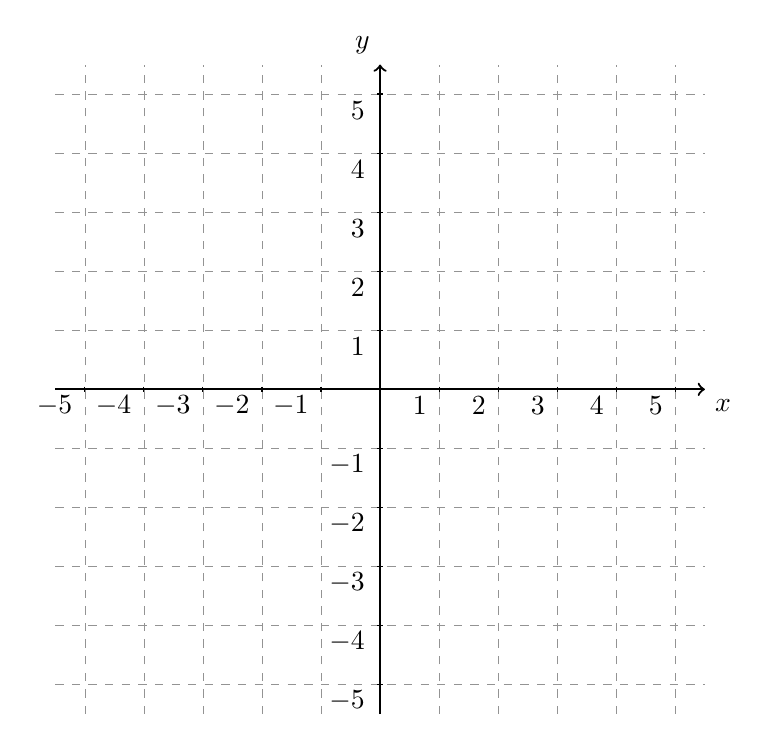
\begin{tikzpicture}[y=0.75cm, x=0.75cm,font=\sffamily]
    % bounds
    % ticks
    \draw[step = 1, gray, very thin,dashed,opacity=0.85] (-5.5, -5.5) grid ( 5.5,5.5);
 	% axis
	\draw[thick,->] (-5.5,0) -- coordinate (x axis mid) (5.5,0) node[anchor = north west] {$x$};
    \draw[thick,->] (0,-5.5) -- coordinate (y axis mid) (0,5.5) node[anchor = south east] {$y$};
    \foreach \y in {-5,-4,...,-1,1,2,...,5.5} {
      \draw (1pt, \y) -- (-1pt, \y) node[yshift=-6,xshift=-1,anchor=east] {$\y$};
    }
    \foreach \x in {-5,-4,...,-1,1,2,...,5.5} {
      \draw (\x,1pt) -- (\x,-1pt) node[yshift=-5,xshift=-1,anchor=east] {$\x$};
    }
  \end{tikzpicture}


\clearpage


\item Determine the $x$ and $y$ intercepts of the following equations.
\begin{enumerate}
\item $x^2+y=9$
  \vfill
\item $y=|x+4|-3$
  \vfill
\end{enumerate}

\item Each of the questions below refers to the equation
  \begin{eqnarray*}
    y & = & |x-2| + h,
  \end{eqnarray*}
  where $h$ is a real number.
  \sideNote{Assume a point is an $x$-intercept and then ask what it
    implies about the resulting equation.}
  \begin{enumerate}
  \item Suppose you know that the graph of the equation has two
    $x$-intercepts. What does this imply about the possible values
    that $h$ could be?
    \vfill
  \item Suppose, instead, you know that the graph of the equation has
    one $x$-intercept. What does this imply about the possible values
    that $h$ could be?
    \vfill
  \item Suppose, instead, you know that the graph of the equation has no
    $x$-intercept. What does this imply about the possible values
    that $h$ could be?
    \vfill
  \end{enumerate}

\clearpage

\item Determine all points lying on the $y$-axis that are 5 units away
  from the point $(4,-2)$.  Use the problem solving process stated
  below, and explicitly identify which part of the process you are
  using in each of your steps.  As a group, write your complete
  solution on the board.


\begin{boxthm}
{\bf Problem Solving Process}
\begin{enumerate}
\item Re-read the problem.
\item Determine what the problem is asking for along with the format of that answer.
\item Circle/Underline the important components of the problem.
\item Determine the topics/concepts being assessed.
\item Write down relevant formulas, definitions, and equations.
\item Discuss your ideas with your group.
\item Make rough sketches of the relationships and try to visualize
  the situation and context.
\item Solve the problem and verify that your solution answers the
  question in the correct format.
\end{enumerate}

\end{boxthm}
\vfill
\clearpage

\item A turtle is in a field. Initially, it is 40 meters north and 60
  meters west of the center of the field.
  \begin{enumerate}
  \item What is the turtle's distance from the center of the field?
    (Make a sketch of the situation using a coordinate system and
    label the axes and important aspects of the graph.)

    \vfill
    \vfill
    
  \item The turtle is moving at a constant speed, and it moves east
    one meter per minute. How far does it move from its initial
    position in $t$ minutes?
    
    \vfill
    
  \item Describe what happens to the turtle's distance from the center
    of the field as time goes by. Do not give an exact answer but give
    a general description of the important trends over time. What
    happens to the distance after a long time?
    
    \vfill

  \item Make a rough sketch of the distance based on your
    description. \sideNote{The graph should not be exact but just
      roughly conveys the important features.}

    \vfill
    \vfill

  \item What is the turtle's location when the distance from the
    center of the field is at its smallest? Are there any times when
    the distance from the center of the field is unique? (i.e. there
    are no other times when the distance is the same.)

    \vfill
    
  \end{enumerate}



\end{enumerate}




\hwTitle{Homework Section 1.1}

\begin{enumerate}
\item The points $ABC$ form a triangle.
  \begin{enumerate}
  \item Plot $A(-1,2),B(3,0) , C(4,2), $ and draw the triangle on the graph below.\\
    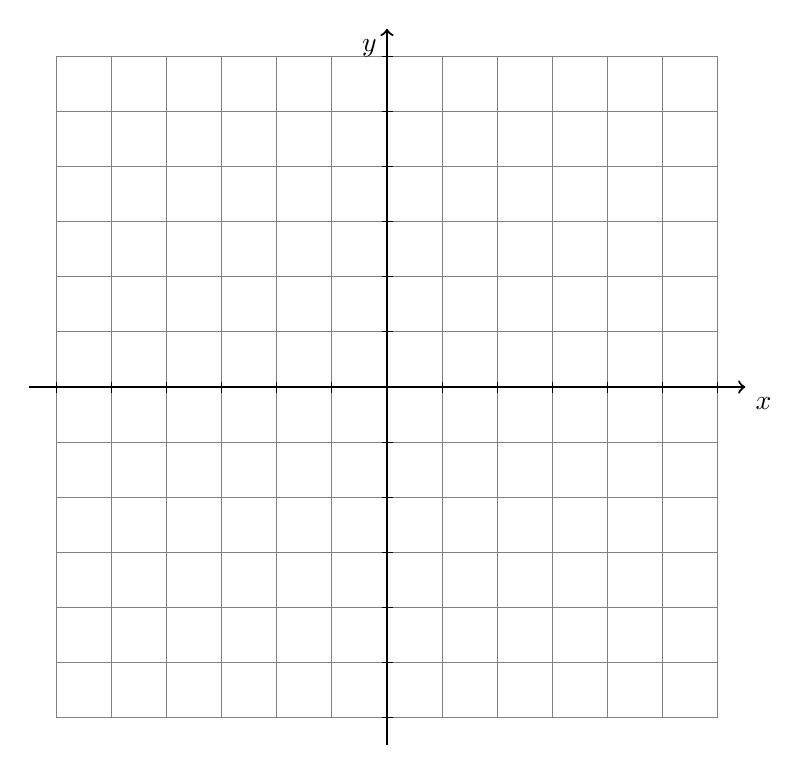
\begin{tikzpicture}[y=.7cm, x=.7cm,font=\sffamily]
      %% ticks
      \draw[step = 1, gray] (-6,-6) grid (6,6);
      %% axis
      \draw[thick,->] (-6.5,0) -- coordinate (x axis mid) (6.5,0) node[anchor = north west] {$x$};
      \draw[thick,->] (0,-6.5) -- coordinate (y axis mid) (0,6.5) node[anchor = north east] {$y$};
      \foreach \y in {-6,-5,...,-1,1,2,...,6} {
        \draw (2pt, \y) -- (-2pt, \y);
      }
      \foreach \x in {-6,-5,...,-1,1,2,...,6} {
        \draw (\x,2pt) -- (\x,-2pt);
      }

    \end{tikzpicture}

  \item Determine the perimeter of the triangle.
  \item Is the triangle a right triangle?  Show work to support your answer.
  \end{enumerate}

\item Use the following parts to find all points on the line $y=2x$ that are 5 units away from $P(-1,3)$.  
  \begin{enumerate}
  \item Find the points $(x,y)$ on the line $y=2x$ for $x=1, -2,$ and $5$.
  \item What if we didn't know the value of $x$?  Write an ordered
    pair formula that works for every point on the line $y=2x$?
  \item Use part (b) to find all points on the line $y=2x$ that are 5 units away from $P(-1,3)$. 
  \end{enumerate}


\item Determine the $x$ and $y$ intercepts of the following equations.
  \begin{enumerate}
  \item $\displaystyle y=3x+10.$
  \item $\displaystyle y=\sqrt{x-10}.$
  \item $\displaystyle y^2 = (x-4)^2.$
  \item $\displaystyle y = x^3 - x.$
  \item $\displaystyle |y-3| = 2|x+1| + 5.$
  \end{enumerate}

\item For each equation below determine all possible values of $x$
  that can be used to calculate a valid value of $y$. Express your
  result three different ways, using interval notation, graphically on
  a line segment, as well as using inequalities.
  \begin{enumerate}
  \item $\displaystyle y=|x+10|.$
  \item $\displaystyle y=\frac{3}{4-x}.$
  \item $\displaystyle y=2x+19.$
  \item $\displaystyle y = \sqrt{x+5}.$
  \item $\displaystyle y = \frac{10}{\sqrt{x+5}}.$
  \end{enumerate}

\item The Racine express is moving straight North out of Chicago, and
  the Davenport Traveler is moving straight West out of Chicago. At a
  given point in time the distance between the trains is four-hundred
  and fifty miles. If the Racine express is ninety miles North of
  Chicago determine the coordinates of the other train. (Treat Chicago
  as the origin.)

\item A rabbit is located in the center of a field. The rabbit's
  burrow is located 20 meters north and 30 meters east of where it is
  currently located. A fox is located 25 meters north and 37 meters
  east of the burrow. If the rabbit can run 11 meters per second and
  the fox can run 13.6 meters per second, can the rabbit reach its
  burrow before the fox reaches the burrow assuming they start running
  at the same time? (Make a sketch of the situation and clearly mark
  the positions of each relevant object.) The time it takes for an
  object moving at a speed of $v$ meters per second to travel $d$
  meters is $\frac{d}{v}$.

  The time it takes for an object moving at a velocity $v$ kph to travel
  $d$ meters 

  \item Mark the point $P_3(1.3,-2.4)$ on the coordinate plane below. Determine the
  points on the $x$-axis that are a distance of 3 units from $P_3$.

  \begin{tikzpicture}[y=1cm, x=1cm,font=\sffamily]
    % bounds
    \def\lowX{-5.5}
    \pgfmathtruncatemacro\startX{round(0.5+\lowX)}
    \pgfmathsetmacro\nextXValue{int(\startX+1)}
    \def\highX{5.5}
    \def\lowY{-5.5}
    \def\highY{5.5}
    \pgfmathsetmacro\nextYValue{int(\lowY+1)}
    % ticks
    \draw[step = 1, gray, very thin,dashed,opacity=0.85] (\lowX, \lowY) grid ( \highX,\highY);
 	% axis
	\draw[thick,->] (\lowX,0) -- coordinate (x axis mid) (\highX,0) node[anchor = north west] {$x$};
    \draw[thick,->] (0,\lowY) -- coordinate (y axis mid) (0,\highY) node[anchor = south east] {$y$};
    \foreach \y in {-5,-4,...,-1,1,2,...,\highY} {
      \draw (1pt, \y) -- (-1pt, \y) node[yshift=-6,xshift=-1,anchor=east] {$\y$};
    }
    \foreach \x in {-5,-4,...,-1,1,2,...,\highX} {
      \draw (\x,1pt) -- (\x,-1pt) node[yshift=-5,xshift=-1,anchor=east] {$\x$};
    }
  \end{tikzpicture}

  \begin{subproblem}
  \item Place points on the graphs near to where you think the points
    \textbf{may} be located.
  \item Label one of the points, $(x,y)$. 
  \item Write out the general distance formula.
  \item What do you know about the point? Can you simplify the formula?
  \item Solve for the unknown variable.
  \end{subproblem}

\end{enumerate}


\preClass{Coordinate Systems}

\videoLink{Section 1.3}{https://www.youtube.com/playlist?list=PLYHZK3b8UFw1_K7VRAlYGdUZOaqjJTOZ\_}

\begin{table}[h]
  \center%
  \begin{tabular}{|l|l|}
    \hline
    \textbf{Actor $x$} & \textbf{Number of Oscar Nominations $y$} \\ \hline
    Tom Hanks          & 5                                        \\ \hline
    Jack Nicholson     & 12                                       \\ \hline
    Sean Penn          & 5                                        \\ \hline
    Dustin Hoffman     & 7                                        \\ \hline
  \end{tabular}
  \label{table:oscarNominations}
  \caption{Number of Oscar nominations for different actors.}
\end{table}



\begin{enumerate}
\item Use the relation given in the table above to answer the following.


\begin{enumerate}
\item Write a set of ordered pairs $(x,y)$ that defines the relation.\vfill
\item Write the domain of the relation.\vfill
\item Write the range of the relation.\vfill
\item Determine if the relation defines $y$ as a function of $x$.
\end{enumerate}
\vfill

\newpage
\item Given $f(x)=x^2+3x$ and $\displaystyle g(x)=\frac{1}{x}$, evaluate the function at the given value of $x$.
\begin{enumerate}
\item $f\left(-2\right)=$
  \vfill
\item $\displaystyle g\left(-\frac{1}{2}\right)=$
  \vfill
\end{enumerate}




\item Express the domain of the functions below three different ways,
  using interval notation, graphically on a line segment, as well as
  using inequalities.
  \begin{enumerate}
  \item $\displaystyle h(x)=\frac{x-3}{x-4}$
    \vfill
  \item $k(x)=\sqrt{x+9}$
    \vfill
  \item $\displaystyle m(x)=\frac{3}{\sqrt{x+9}}$
    \vfill
  \end{enumerate}





\end{enumerate}






\actTitle{Worksheet 1.3}

\noindent
Student goals:
  \begin{itemize}
  \item Determine if a given description of a relationship is a
    function using written, graphical, and tabular descriptions.
  \item Use correct notation to describe a function and be able to
    identify the order of operations in a given expression.
  \item Compute values of a given function.
  \item Make a rough sketch of the graph of a function.
  \item Determine domain or range given a graphical, algebraic, or
    tabular representation of a function.
  \item Determine a function given a written description of a
    situation or context.
  \item Determine intervals in the domain where a function is
    increasing/decreasing/constant
  \end{itemize}


\noindent \textbf{Instructions:}  Work together in groups of  3 or 4 to complete the following problems.


\begin{enumerate}

\item Answer True or False to each statement below and provide a
  justification for your answer.
\begin{enumerate}
%\item $x=2$ is in the domain of $\displaystyle f(x)=\frac{x-2}{3x+1}$.
%\vfill
%\item $x=\frac{1}{3}$ is in the domain of $\displaystyle f(x)=\frac{x-2}{3x+1}$.
\item $x=-\frac{1}{3}$ is in the domain of $\displaystyle f(x)=\frac{x-2}{3x+1}$.
  \vfill
\item $x=-3$ is in the domain of $\displaystyle f(x)=\sqrt{x+3}$.
  \vfill
\item $x=-4$ is in the domain of $\displaystyle f(x)=\sqrt{x+3}$.
  \vfill
\end{enumerate}

\clearpage

\item The graphs for different functions are given below. For each
  function state the domain and range of the function using interval
  notation. Also, state the values of $x$ where the functions are
  increasing and where they are decreasing. Finally, state whether or
  not there are any values of $y$ for which the value of the function
  is equal to $y$ for more than one value of $x$.

\begin{enumerate}
\item 
\begin{center}
	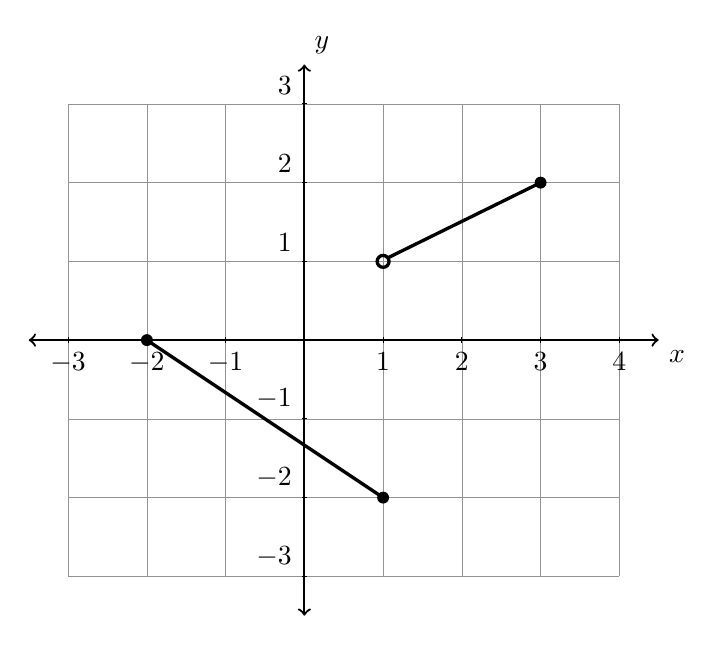
\begin{tikzpicture}[y=1.0cm, x=1.0cm,font=\sffamily,
  mydot/.style={
    circle,
    fill=white,
    draw,
    outer sep=0pt,
    inner sep=1.5pt
  }]
    %% Add a grid
    \draw[step = 1, gray, very thin,opacity=0.85] (-3, -3) grid ( 4, 3);
 	%% Draw the axes
	\draw[thick,<->] (-3.5,0) -- coordinate (x axis mid) (4.5,0) node[anchor = north west] {$x$};
    \draw[thick,<->] (0,-3.5) -- coordinate (y axis mid) (0,3.5) node[anchor = south west] {$y$};
    %% Label the y axis
    \foreach \y in {-3,-2,-1,1,2,...,3} {
      \draw (1pt, \y) -- (-1pt, \y) node[anchor = south east] {$\y$};
    }
    %% Label the x axis
    \foreach \x in {-3,...,-1,1,2,...,4} {
      \draw (\x,1pt) -- (\x,-1pt) node[anchor = north] {$\x$};
    }
    %% Draw the function.
    \begin{scope}
         \draw[scale=1.0,very thick,black] (-2, 0) -- (1,-2);
         \draw[scale=1.0,very thick,black] (1.05,1.04) -- (3,2);
         \fill[black] (-2, 0) circle[radius=0.5ex];
         \fill[black] (3,2) circle[radius=0.5ex];
         \fill[black] (1,-2) circle[radius=0.5ex];
         \draw[scale=1.0, very thick, black] (1,1) circle[radius=0.5ex];

    \end{scope}

    %%\node[above=0.1cm] at (-2,2 )   {\nextXValue};

  \end{tikzpicture}
\end{center}

\vfill

\item
\begin{center}
	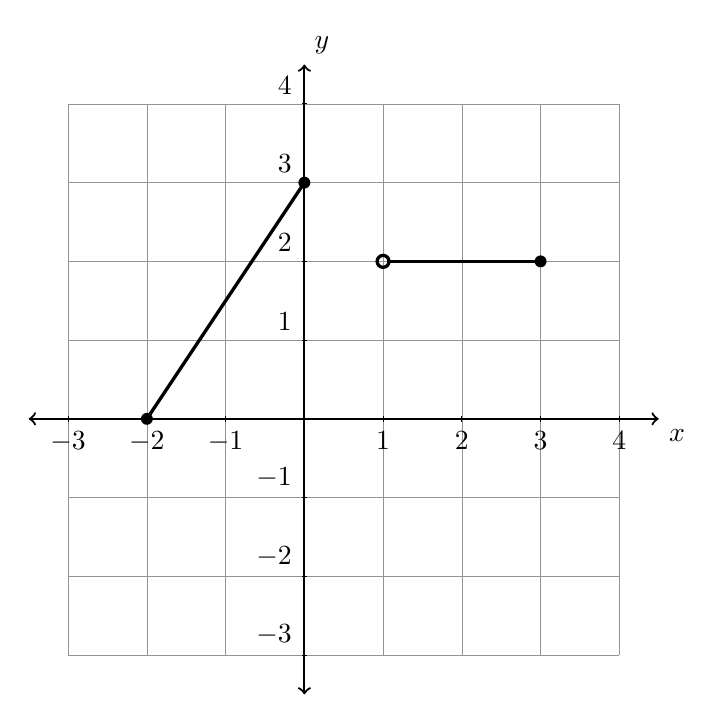
\begin{tikzpicture}[y=1.0cm, x=1.0cm,font=\sffamily,
  mydot/.style={
    circle,
    fill=white,
    draw,
    outer sep=0pt,
    inner sep=1.5pt
  }]
    %% Add a grid
    \draw[step = 1, gray, very thin,opacity=0.85] (-3, -3) grid ( 4, 4);
 	%% Draw the axes
	\draw[thick,<->] (-3.5,0) -- coordinate (x axis mid) (4.5,0) node[anchor = north west] {$x$};
    \draw[thick,<->] (0,-3.5) -- coordinate (y axis mid) (0,4.5) node[anchor = south west] {$y$};
    %% Label the y axis
    \foreach \y in {-3,-2,-1,1,2,...,3,4} {
      \draw (1pt, \y) -- (-1pt, \y) node[anchor = south east] {$\y$};
    }
    %% Label the x axis
    \foreach \x in {-3,...,-1,1,2,...,4} {
      \draw (\x,1pt) -- (\x,-1pt) node[anchor = north] {$\x$};
    }
    %% Draw the function.
    \begin{scope}
         \draw[scale=1.0,very thick,black] (-2, 0) -- (0,3);
         \draw[scale=1.0,very thick,black] (1.05,2) -- (3,2);
         \fill[black] (-2, 0) circle[radius=0.5ex];
         \fill[black] (3,2) circle[radius=0.5ex];
         \fill[black] (0,3) circle[radius=0.5ex];
         \draw[scale=1.0, very thick, black] (1,2) circle[radius=0.5ex];

    \end{scope}

    %%\node[above=0.1cm] at (-2,2 )   {\nextXValue};

  \end{tikzpicture}
\end{center}

\vfill

\end{enumerate}

\clearpage

\item Determine the domain of each of the following functions. Give
  your answer in interval notation as well as sketching a graph of the
  real number line showing the domain graphically.
\begin{enumerate}
\item $g(x) = x^2$
  \vfill
\item $f(x)=\sqrt{3x-7}$
  \vfill
%\item $f(x) = \dfrac{x+3}{x^2-9}$
\item $h(x)=\dfrac{5}{x^2-25}$
  \vfill
\item $f(x) = \sqrt{x^2-4x+3}$
  \sideNote{Make a sketch of the quadratic function without the square
    root first.}
  \vfill
  \vfill
\item $g(x) = \dfrac{\sqrt{x^2-4x+3}}{x^3+8}$
  \vfill

\end{enumerate}

\clearpage

\item The graph of different relationships are given in the figures
  below. For each relationship determine whether or not the
  relationship is a function. Provide specific reasons for your
  conclusion and do not just cite the name of a particular rule or
  test. Also, state all of the intercepts for each relationship.

  \begin{enumerate}
  \item
  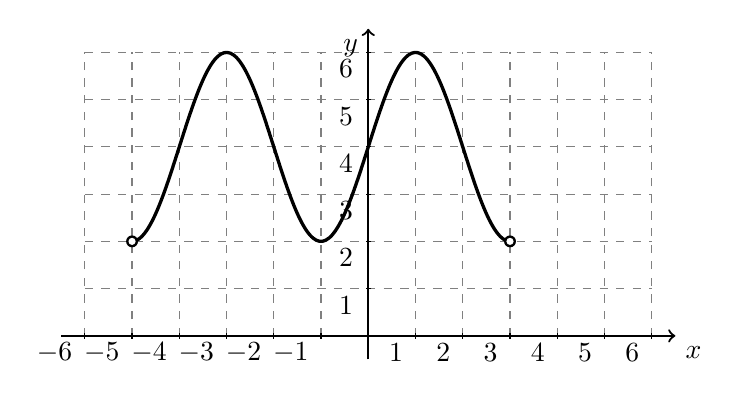
\begin{tikzpicture}[y=0.6cm, x=0.6cm,font=\sffamily]
    %% ticks
    \draw[step = 1, gray,dashed] (-6,0) grid (6,6);
    %% axis
    \draw[thick,->] (-6.5,0) -- coordinate (x axis mid) (6.5,0) node[anchor = north west] {$x$};
    \draw[thick,->] (0,-.5) -- coordinate (y axis mid) (0,6.5) node[anchor = north east] {$y$};
    \foreach \y in {1,2,...,6} {
      \draw (1pt, \y) -- (-1pt, \y) node[yshift=-6,xshift=-1,anchor=east] {$\y$};
    }
    \foreach \x in {-6,-5,...,-1,1,2,...,6} {
      \draw (\x,1pt) -- (\x,-1pt) node[yshift=-5,xshift=-1,anchor=east] {$\x$};
    }

    \begin{scope}
      %\clip(-4,-1) rectangle (8,5);
      \draw[scale=1.0,domain=-4:4,smooth,variable=\x,very thick,black,samples=120] 
           plot ({\x-1},{4+2*sin(deg(pi*\x/2-pi/2))});
      \fill[black] (-5,2) circle [radius=0.5ex];
      \fill[white] (-5,2) circle [radius=0.3ex];
      \fill[black] ( 3,2) circle [radius=0.5ex];
      \fill[white] ( 3,2) circle [radius=0.3ex];
    \end{scope}

  \end{tikzpicture}

  \item 
    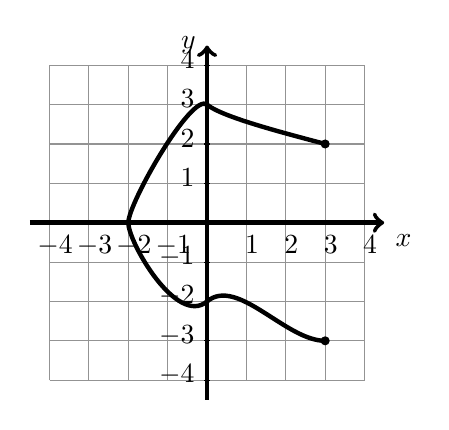
\begin{tikzpicture}[y=0.5cm, x=0.5cm,font=\sffamily]
      \draw[step = 1, gray, thin,opacity=0.85] (-4,-4) grid (4,4);
      \draw[black,ultra thick,->] (-4.5,0) -- (4.5,0) node[anchor=north west] {$x$};
      \draw[black,ultra thick,->] (0,-4.5) -- (0,4.5) node[anchor=east] {$y$};
      \foreach \y in {-4,-3,-2,-1,1,2,3,4} {
        \draw (1pt, \y) -- (-1pt, \y) node[anchor = east,yshift=2] {$\y$};
        \draw (\y,1pt) -- (\y,-1pt) node[anchor = north,xshift=2] {$\y$};
      }
      \draw[ultra thick,black] (3, -3) .. controls +(0:-1) and +(40:1) .. (0, -2)
                    ( 0,-2) .. controls +( 40:-1.0) and +(90:-0.5) .. (-2, 0)
                    (-2, 0) .. controls +( 90:0.5) and +(-40:-0.5) .. (0,3)
                    ( 0, 3) .. controls +(-40:0.5) and +(-15:-1) .. (3, 2);
          \draw[black,fill=black]  (3,-3) circle (0.1);
          \draw[black,fill=black]  (3, 2) circle (0.1);

    \end{tikzpicture}
  \end{enumerate}
  
  \clearpage


\end{enumerate}

\hwTitle{Section 1.3}

\begin{enumerate}
\item The Racine express is moving straight North out of Chicago at a
  speed of 80 kilometers per hour. The Davenport Traveler is moving
  straight West out of Chicago at a speed of 90 kilometers per
  hour. The trains leave the station at the same time. Determine an
  equation for the distance between the two trains as a function of
  time.

\item Consider the relation that is defined by taking an object on
  your desk and assigning to it its color.  For example, if there is a
  hat on your desk that is green and blue, we would write
  $$f(\text{hat}) = \{\text{green, blue}\}.$$
  If there is a pen on your desk that is red, we would write
  $$f(\text{pen}) = \text{red}.$$
\begin{enumerate}
\item List at least three items on your desk and come up with your own
  relation. (You can use imaginary items or objects in the room, if
  you need to.)
\item What is the domain and range of your relation?
\item Is your relation a function?  Why or why not?
\end{enumerate}

\item Determine the domain of each of the following functions. Give your answer in interval notation.%\\[.5in]
\begin{enumerate}
\item $g(x) = x^3$
\item $f(x)=\sqrt{x+1}$
\item $h(x)=\frac{5}{x-4}$
\item $k(x) = \dfrac{x+3}{x^2-9}$
\item $l(x)=\dfrac{1}{x^2+1}$
\item $m(x) = \sqrt{x^2-2x-15}$
\item $n(x) = \frac{1}{\sqrt{x^2-2x-15}}$
\end{enumerate}

\item Use the axes below to make a rough sketch of each of the
  indicated functions.
  \pagebreak[4]
  \begin{enumerate}

  \item ${\displaystyle y=x^2}$
\begin{center}
	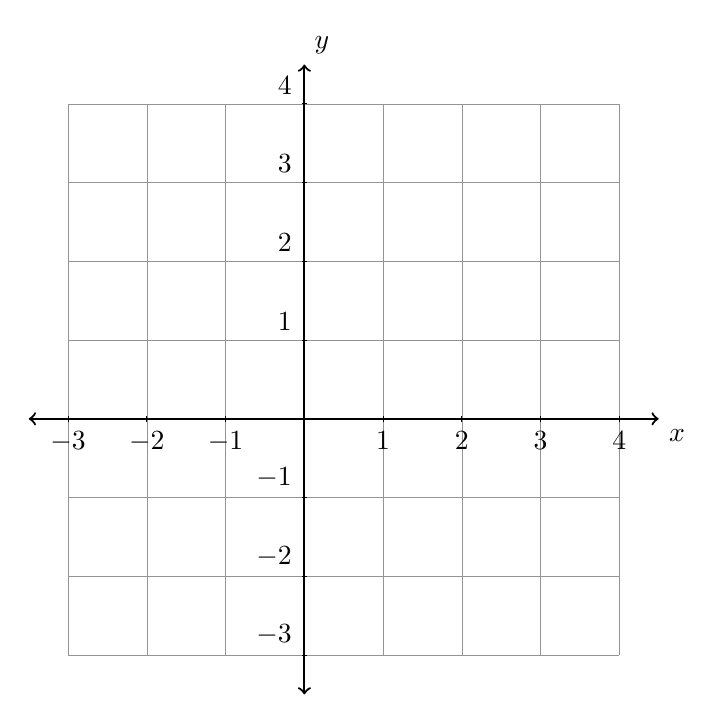
\begin{tikzpicture}[y=1.0cm, x=1.0cm,font=\sffamily,
  mydot/.style={
    circle,
    fill=white,
    draw,
    outer sep=0pt,
    inner sep=1.5pt
  }]
    %% Add a grid
    \draw[step = 1, gray, very thin,opacity=0.85] (-3, -3) grid ( 4, 4);
 	%% Draw the axes
	\draw[thick,<->] (-3.5,0) -- coordinate (x axis mid) (4.5,0) node[anchor = north west] {$x$};
    \draw[thick,<->] (0,-3.5) -- coordinate (y axis mid) (0,4.5) node[anchor = south west] {$y$};
    %% Label the y axis
    \foreach \y in {-3,-2,-1,1,2,...,3,4} {
      \draw (1pt, \y) -- (-1pt, \y) node[anchor = south east] {$\y$};
    }
    %% Label the x axis
    \foreach \x in {-3,...,-1,1,2,...,4} {
      \draw (\x,1pt) -- (\x,-1pt) node[anchor = north] {$\x$};
    }
  \end{tikzpicture}
\end{center}

\item ${\displaystyle y=x}$
\begin{center}
	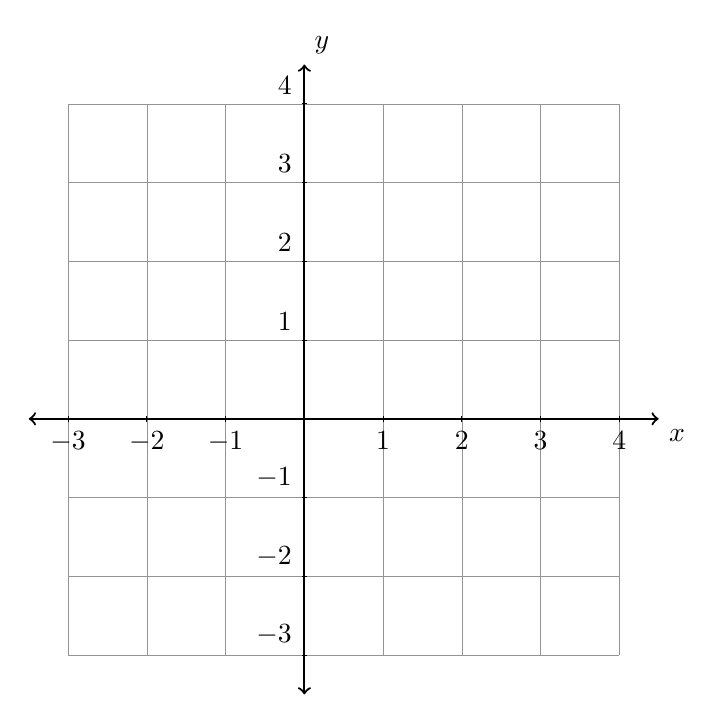
\begin{tikzpicture}[y=1.0cm, x=1.0cm,font=\sffamily,
  mydot/.style={
    circle,
    fill=white,
    draw,
    outer sep=0pt,
    inner sep=1.5pt
  }]
    %% Add a grid
    \draw[step = 1, gray, very thin,opacity=0.85] (-3, -3) grid ( 4, 4);
 	%% Draw the axes
	\draw[thick,<->] (-3.5,0) -- coordinate (x axis mid) (4.5,0) node[anchor = north west] {$x$};
    \draw[thick,<->] (0,-3.5) -- coordinate (y axis mid) (0,4.5) node[anchor = south west] {$y$};
    %% Label the y axis
    \foreach \y in {-3,-2,-1,1,2,...,3,4} {
      \draw (1pt, \y) -- (-1pt, \y) node[anchor = south east] {$\y$};
    }
    %% Label the x axis
    \foreach \x in {-3,...,-1,1,2,...,4} {
      \draw (\x,1pt) -- (\x,-1pt) node[anchor = north] {$\x$};
    }
  \end{tikzpicture}
\end{center}

\pagebreak[4]

\item ${\displaystyle y=\sqrt{x}}$ 
\begin{center}
	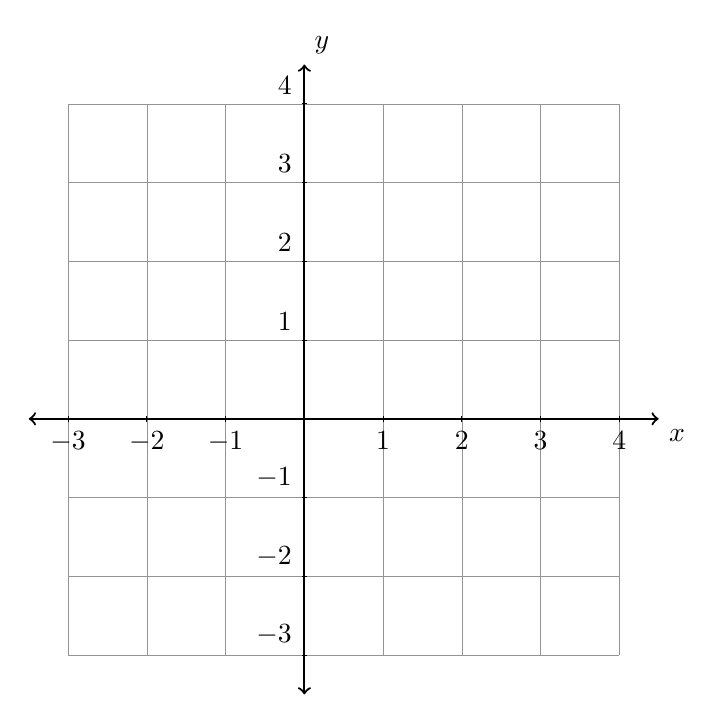
\begin{tikzpicture}[y=1.0cm, x=1.0cm,font=\sffamily,
  mydot/.style={
    circle,
    fill=white,
    draw,
    outer sep=0pt,
    inner sep=1.5pt
  }]
    %% Add a grid
    \draw[step = 1, gray, very thin,opacity=0.85] (-3, -3) grid ( 4, 4);
 	%% Draw the axes
	\draw[thick,<->] (-3.5,0) -- coordinate (x axis mid) (4.5,0) node[anchor = north west] {$x$};
    \draw[thick,<->] (0,-3.5) -- coordinate (y axis mid) (0,4.5) node[anchor = south west] {$y$};
    %% Label the y axis
    \foreach \y in {-3,-2,-1,1,2,...,3,4} {
      \draw (1pt, \y) -- (-1pt, \y) node[anchor = south east] {$\y$};
    }
    %% Label the x axis
    \foreach \x in {-3,...,-1,1,2,...,4} {
      \draw (\x,1pt) -- (\x,-1pt) node[anchor = north] {$\x$};
    }
  \end{tikzpicture}
\end{center}

\item ${\displaystyle y=\frac{1}{x}}$
  \nopagebreak[4]
\begin{center}
	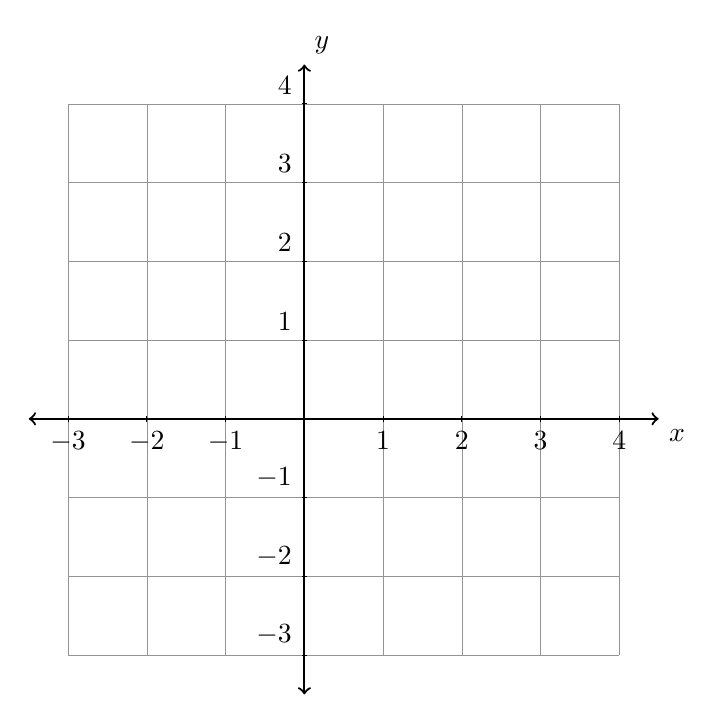
\begin{tikzpicture}[y=1.0cm, x=1.0cm,font=\sffamily,
  mydot/.style={
    circle,
    fill=white,
    draw,
    outer sep=0pt,
    inner sep=1.5pt
  }]
    %% Add a grid
    \draw[step = 1, gray, very thin,opacity=0.85] (-3, -3) grid ( 4, 4);
 	%% Draw the axes
	\draw[thick,<->] (-3.5,0) -- coordinate (x axis mid) (4.5,0) node[anchor = north west] {$x$};
    \draw[thick,<->] (0,-3.5) -- coordinate (y axis mid) (0,4.5) node[anchor = south west] {$y$};
    %% Label the y axis
    \foreach \y in {-3,-2,-1,1,2,...,3,4} {
      \draw (1pt, \y) -- (-1pt, \y) node[anchor = south east] {$\y$};
    }
    %% Label the x axis
    \foreach \x in {-3,...,-1,1,2,...,4} {
      \draw (\x,1pt) -- (\x,-1pt) node[anchor = north] {$\x$};
    }
  \end{tikzpicture}
\end{center}

\end{enumerate}




\end{enumerate}


\preClass{Coordinate Systems}



\noindent Watch the Pre-Class videos for Section 1.4 and answer the following questions. Remember that in your written work you are graded on the correctness of your supporting work and not just your final answer. Always give an exact answer unless you are explicitly told to round; calculator approximations will not receive full credit. 


\begin{enumerate}
\item  Determine a \emph{point-slope} equation for a line through $(-5,2)$ and $(6,-3)$.

\vfill
\item Write the \emph{slope-intercept} equation for a line through the point $(2,3)$ that is perpendicular to the line $2x+4y-7=0$.

\vfill


\item Given the function defined $f(x)=x^2+3$, determine the average rate of change of $f(x)$ from $x_1=2$ to $x_2=4$.
\vfill

\end{enumerate}






\actTitle{Worksheet 1.4}


\noindent \textbf{Instructions:}  Work together in groups of  3 or 4 to complete the following problems.

\noindent
Student goals:
\begin{itemize}
\item Define a linear relationship from a written description.
\item Determine the slope of a line from a written description or an algebraic expression.
\item Compare the slopes of lines and interpret relative steepness as well as interpret positive versus negative slope.
\item Calculate the average rate of change between two points on a function.
\item Determine algebraic expressions for horizontal and vertical lines.
\item Translate the formulae for lines between slope-intercept,
  point slope, and general forms.
\end{itemize}



\begin{enumerate}
\item Let $f(x)$ be a linear function such that $\displaystyle f(2)=\frac{7}{3}$ and the graph of $f(x)$ is parallel to the line $2x+3y+4=0$. 
\begin{enumerate}
\item Determine $f(x)$ and write your final answer in \emph{slope-intercept} form. (Leave fractions in your answer, no decimals.)
\vfill
\item Graph $f(x)$ and  $2x+3y+4=0$ on the rectangular coordinate system below.\\
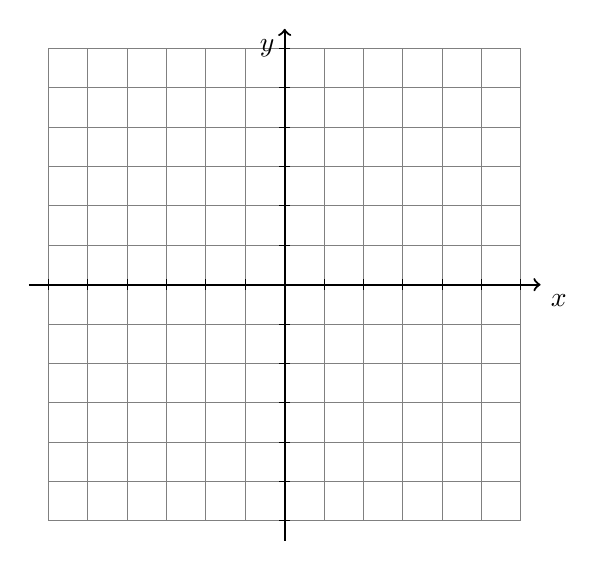
\begin{tikzpicture}[y=.5cm, x=0.5cm,font=\sffamily]
    %% ticks
    \draw[step = 1, gray] (-6,-6) grid (6,6);
    %% axis
    \draw[thick,->] (-6.5,0) -- coordinate (x axis mid) (6.5,0) node[anchor = north west] {$x$};
    \draw[thick,->] (0,-6.5) -- coordinate (y axis mid) (0,6.5) node[anchor = north east] {$y$};
    \foreach \y in {-6,-5,...,-1,1,2,...,6} {
      \draw (2pt, \y) -- (-2pt, \y);
    }
    \foreach \x in {-6,-5,...,-1,1,2,...,6} {
      \draw (\x,2pt) -- (\x,-2pt);
    }

  \end{tikzpicture}

\item Determine the domain and range of $f(x)$.\\[.5in]
\end{enumerate}


\newpage
\item Determine whether the lines $y= 2x+3$ and and $x-3y-5=0$ are parallel, perpendicular, or neither. \vfill


\item Determine an equation of the \emph{vertical} line which passes through the point $(-2, 3)$. Then determine an equation of the \emph{horizontal} line through $(-2,3)$.\vfill

\newpage

\item Consider the function $f(x)=x^2-3x+2$.
\begin{enumerate}
\item Algebraically determine the average rate of change of $f(x)=x^2-3x+2$ between $x_1=1$ and $x_2=3$.
\vfill



\item The graph of $f(x)=x^2-3x+2$ is given below.  Draw a line between the points $(1,f(1))$ and $(3,f(3))$.\\

%\begin{tikzpicture}[scale=1]
%	\begin{axis}[
%	                   axis equal,
%	                   axis line style = thick,
%	                   axis x line=middle, 
%	                   axis y line=center, 
%	                   minor tick num = 3,
%	                   grid = both,
%	                   major grid style={black!70},
%	                   minor grid style ={gray!70},
%	                   xtick={-4,-2,0,2,4,6},
%	                   ytick={-2,0,2,4,6,8},
%	                   xmin = -4,
%	                   xmax = 6,
%	                   ymin = -2.25,
%	                   ymax = 8.25,
%	                   tick align=outside,
%	                   style={font=\tiny}]
%
%		\addplot+[mark=none,smooth, style={thick}] (\x,{\x*\x-3*\x+2});
%		\addplot[only marks, style={mark size=1pt}] table {
%		0 2
%		1 0
%		1.5 -.25 
%		2 0
%		};
%	\end{axis}
%\end{tikzpicture}

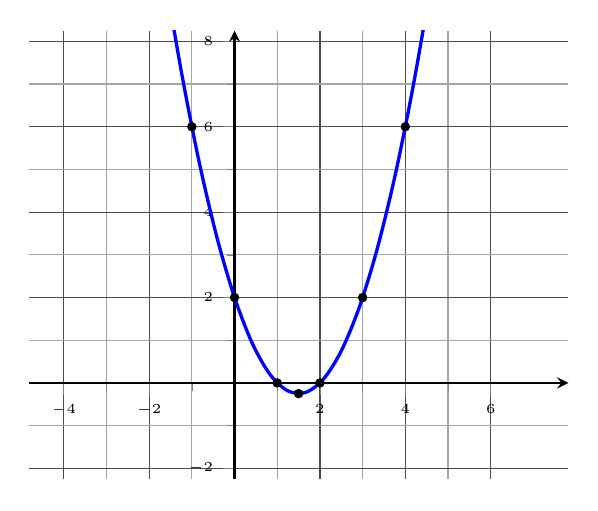
\begin{tikzpicture}[scale=1]
	\begin{axis}[
	                   axis equal,
	                   axis line style = thick,
	                   axis x line=middle, 
	                   axis y line=center, 
	                   minor tick num = 1,
	                   grid = both,
	                   major grid style={black!70},
	                   minor grid style ={gray!70},
	                   xtick={-4,-2,0,2,4,6},
	                   ytick={-2,0,2,4,6,8},
	                   xmin = -3,
	                   xmax = 6,
	                   ymin = -2.25,
	                   ymax = 8.25,
	                   tick align=outside,
	                   style={font=\tiny}]

		\addplot+[mark=none,smooth, style={very thick}] (\x,{\x*\x-3*\x+2});
		\addplot[only marks, style={mark size=1.5pt}] table {
		0 2
		1 0
		1.5 -.25 
		2 0
		3 2
		4 6
		-1 6
		};
	\end{axis}
\end{tikzpicture}

\item Find the slope of the line between the points $(1,f(1))$ and $(3,f(3))$ on $f(x)=x^2-3x+2$.
\vfill
\item What do you notice about the slope of the line between the
  points $(1,f(1))$ and $(3,f(3))$ on $f(x)=x^2-3x+2$ and the average
  rate of change of $f(x)=x^2-3x+2$ between $x_1=1$ and $x_2=3$.
  Why is this?
\end{enumerate}

\clearpage

\item The equations for two different lines are the
  following:
  \begin{eqnarray*}
    \mathrm{Line~1:~} y-3 & = & 4 (x-2), \\
    \mathrm{Line~2:~} y-2 & = & m (x-1),
  \end{eqnarray*}
  where $m$ is a real-valued number.

  \begin{enumerate}
  \item What are the possible values of $m$ that will ensure that the
    two lines intersect? (Provide a justification for your answer.)

    \vfill
  
  \item If you are given that the values of $y$ for the points on the
    graph of line 2 are greater than those of line 1 when $x$ is positive
    what does that imply about the possible values that $m$ could be?
    (Provide a justification for your answer.)
    \sideNote{Make a rough sketch of the graphs representing this situation.}

    \vfill

  \item What values of $m$ will ensure that the $y$ values on the
    graph of line 1 will be less that those on the graph of line 2
    when $x>3$?

    \vfill

  \end{enumerate}



\end{enumerate}



\hwTitle{Section 1.4}

\begin{enumerate}
\item Consider the line $x+2y=3$.
  \begin{enumerate}
  \item Find the $x$ and $y$ intercepts of the line.
  \item Determine the distance between the $x$-intercept and the $y$-intercept.
  \item Find the slope of the line $x+2y=3$.
  \end{enumerate}

\item The questions below refer to the linear functions shown in the
  plot below. The function $f(x)=m_f x + b_f$ is shown with a solid
  line, the function $g(x)=m_g x + b_g$ is shown with a dashed line,
  and the function $h(x) = m_h x + b_h$ is shown with a dotted line.

  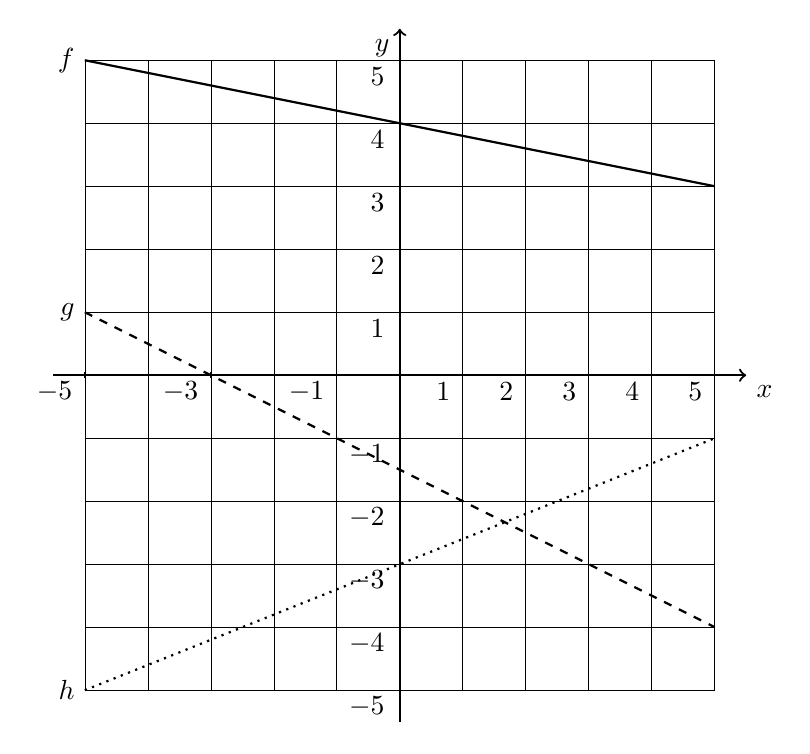
\begin{tikzpicture}[y=0.8cm, x=0.8cm,font=\sffamily]
    %% ticks
    \draw[step = 1, very thin] (-5, -5) grid ( 5,5);
    % axis
    \draw[thick,->] (-5.5,0) -- coordinate (x axis mid) (5.5,0) node[anchor = north west] {$x$};
    \draw[thick,->] (0,-5.5) -- coordinate (y axis mid) (0,5.5) node[anchor = north east] {$y$};
    \foreach \y in {-5,-4,...,-1,1,2,...,5} {
      \draw (1pt, \y) -- (-1pt, \y) node[yshift=-6,xshift=-1,anchor=east] {$\y$};
    }
    \foreach \x in {-5,-3,...,-1,1,2,...,5} {
      \draw (\x,1pt) -- (\x,-1pt) node[yshift=-5,xshift=-1,anchor=east] {$\x$};
    }

    \begin{scope}
      %\clip(-4,-1) rectangle (8,5);
      \draw[thick,solid]  (-5, 5) node[anchor = east] {$f$}  -- (5, 3);
      \draw[thick,dashed] (-5, 1) node[anchor = east] {$g$}  -- (5,-4);
      \draw[thick,dotted] (-5,-5) node[anchor = east] {$h$}  -- (5,-1);
    \end{scope}

  \end{tikzpicture}

  \begin{enumerate}
    \item Determine which $y$-intercept ($b_f$, $b_g$, and $b_h$)
    is the largest and which is the lowest. (Recall that a negative
    number is less than a positive number.) Provide a brief
    justification for your conclusion based on the graph.

    \item Determine which slopes ($m_f$, $m_g$, and $m_h$) is the
    largest and which is the lowest.  Provide a brief justification
    for your conclusion based on the graph.

    \item Determine which function has the highest $x$-intercept
    and which function has the lowest $x$-intercept. Provide a brief
    justification for your conclusion based on the graph.

  \end{enumerate}

\item The equations for two different linear functions are the
  following:
  \begin{eqnarray*}
    \mathrm{Line~1:~} A(x) & = & 5(x+1)-7, \\
    \mathrm{Line~2:~} B(x) & = & m(x+1)-6,
  \end{eqnarray*}
  where $m$ is a constant. Answer each question below and provide
  a brief justification for your answer.

  \begin{enumerate}
  \item For what values of $m$ does the function $B(x)$ increase?
  \item For what values of $m$ does the function $B(x)$ decrease?
  \item For what values of $m$ do the two lines intersect?
  \item For what values of $m$ is $A(x)>B(x)$ for positive values of
    $x$?
  \item For what values of $m$ is $A(x)<B(x)$ for positive values of
    $x$?
  \end{enumerate}

\end{enumerate}


\preClass{Coordinate Systems}

\videoLink{Section 1.5}{https://www.youtube.com/playlist?list=PLYHZK3b8UFw0ZgjxBc6v6QlaHhSZheL-B}



\begin{enumerate}
\item A sales person makes a base salary of \$350 per week plus 15\% commission on sales.
\begin{enumerate}
\item Write a linear function to model the sales person's weekly salary $S(x)$ for $x$ dollars in sales.\vfill
\item Evaluate $S(700)$ and interpret the meaning in the context of this problem.
\end{enumerate}

\vfill
\item A town's population has been growing linearly. On January 1,
  2004 the population was 6,200. By July 1, 2009 the population had
  grown to 8,100. Assume this trend continues.

\begin{enumerate}
\item The town's population is a function of time, and a coordinate on
  the graph of the function can be written in the form $(t,P)$, where
  $t$ is the number of years since January 1, 2004 and $P$ is the
  population at the given time. From the statement above determine two
  points that will be on the graph of the function.
  
  \vspace{2em}

\item Use the points to determine a linear model for this data.
  
  \vfill

\item Interpret the meaning of the slope in this context.
  
\end{enumerate}

\vfill

\textit{(Continued on next page)}

\clearpage

\item A small animal moves along a wall and starts at a position 3.5
  meters from a corner.  The animal travels 0.3 meters away from the
  corner each minute. Determine the function that provides the
  distance the animal is from the corner given the number of minutes
  from the initial time. What are the units of the slope?

  \vfill

\item A manufacturing facility has 3.5 litres of a material available
  at the start of a given days. The facility produces 0.3 litres of
  material each hour. Determine the function that provides the amount
  of material available given the number of hours from the initial
  time. What are the units of the slope?

  \vfill




\end{enumerate}






\actTitle{Worksheet 1.5}


\noindent \textbf{Instructions:}  Work together in groups of  3 or 4 to complete the following problems.




\begin{enumerate}

\item A small business makes cookies and sells them at the farmer's market.  The fixed monthly cost for use of a Health Department-approved kitchen and rental space at the farmer's market is \$790.  The cost of labor, taxes, and ingredients for the cookies amounts to \$0.24 per cookie, and the cookies sell for \$6.00 per dozen.
\begin{enumerate}
\item Write a linear cost function representing the cost $C(x)$ to produce $x$ dozen cookies per month.  Then determine the monthly cost to produce 100 dozen cookies each month.
\vfill
\item Write a linear revenue function representing the revenue $R(x)$ for selling $x$ dozen cookies.  Then determine the revenue for for selling 100 dozen cookies.
\vfill
\item Will the business make a profit or lose money if they sell 100 dozen cookies each month?
\vfill
\item Write a linear profit function representing the profit $P(x)$ for producing and selling $x$ dozen cookies in a month. (Profit is revenue minus cost.)
\vfill
\item Determine the least number of cookies (in dozens) that must be produced and sold for a monthly profit.  Your answer should be an appropriate whole number.
\vfill
\item If 150 dozen cookies are sold in a given month, how much money will the business make or lose?
\vfill
\end{enumerate}

\newpage

\item The boiling point of water is 212$^\circ$ Fahrenheit and 100$^\circ$ Celsius. The freezing point of water
 is 32$^\circ$ Fahrenheit and 0$^\circ$ Celsius. Fahrenheit and Celsius are linearly related.
 
 \begin{enumerate}
 \item Determine a function that will tell you the temperature in degrees Celsius if
you already know the temperature in degrees Fahrenheit.
\vfill
\vfill
 \item If it is 83$^\circ$ Fahrenheit, determine the temperature in degrees Celsius.
 \end{enumerate}
 \vfill
 
 \item A car has a 15-gal tank for gasoline and gets 30 mpg on a highway while driving 60 mph. Suppose that the driver starts a trip with a full tank of gas and travels 450 mi on the highway at an average speed of 60 mph.
 
 \begin{enumerate}
 \item Write a linear model representing the amount of gas $G(t)$ left in the tank t hours into the trip.
 \vfill
 \vfill
 \item Evaluate $G(4.5)$ and interpret the meaning in the context of the problem.
 \vfill
 \end{enumerate}
 
 \newpage
 

\item The table gives the number of calories and the amount of cholesterol for selected fast food hamburgers.\\
\begin{table}[h]
\begin{tabular}{|l|l|}
\hline
\textbf{Hamburger Calories} & \textbf{Cholesterol (mg)} \\ \hline
220                         & 35                        \\ \hline
420                         & 50                        \\ \hline
460                         & 50                        \\ \hline
480                         & 60                        \\ \hline
560                         & 70                        \\ \hline
590                         & 105                       \\ \hline
610                         & 65                        \\ \hline
680                         & 80                        \\ \hline
720                         & 90                        \\ \hline
\end{tabular}
\end{table}
\begin{enumerate}
\item Use the data points (480,60) and (720,90) to write a linear function that defines the amount of cholesteral $c(x)$ as a linear function of the number of calories $x$.
\vfill
\item Interpret the meaning of the slope in the context of this problem.
\vfill
\item Use the model from part (a) to predict the amount of cholesterol for a hamburger with 650 calories.  
\vfill
\end{enumerate}

%\newpage
%
%
%\item Given a square with sides of length $s$, diagonal of length $d$, perimeter $P$, and area $A$,
%\begin{enumerate}
%
%\item Write $P$ a function of $s$.
%\vfill
%\item Write $A$ as a function of $s$.
%\vfill
%\item Write $A$ as a function of $P$.
%\vfill
%\item Write $P$ as a function of $A$.
%\vfill
%\item Write $d$ as a function of $s$.
%\vfill
%\item Write $s$ as a function of $d$.
%\vfill
%\item Write $P$ as a function of $d$.
%\vfill
%\item Write $A$ as a function of $d$.
%\vfill
%
%\end{enumerate}
\end{enumerate}


















\preClass{Coordinate Systems}


\videoLink{Section 1.6 Day 1}{https://www.youtube.com/playlist?list=PLYHZK3b8UFw3srUWdN3pnV1WRNsEcqx-T}


\begin{enumerate}

\item  For this problem, let $f(x)=|x|$.

\begin{enumerate}
\item Graph $f(x)=|x|$.  Then determine the domain and range of $f(x)$.\\
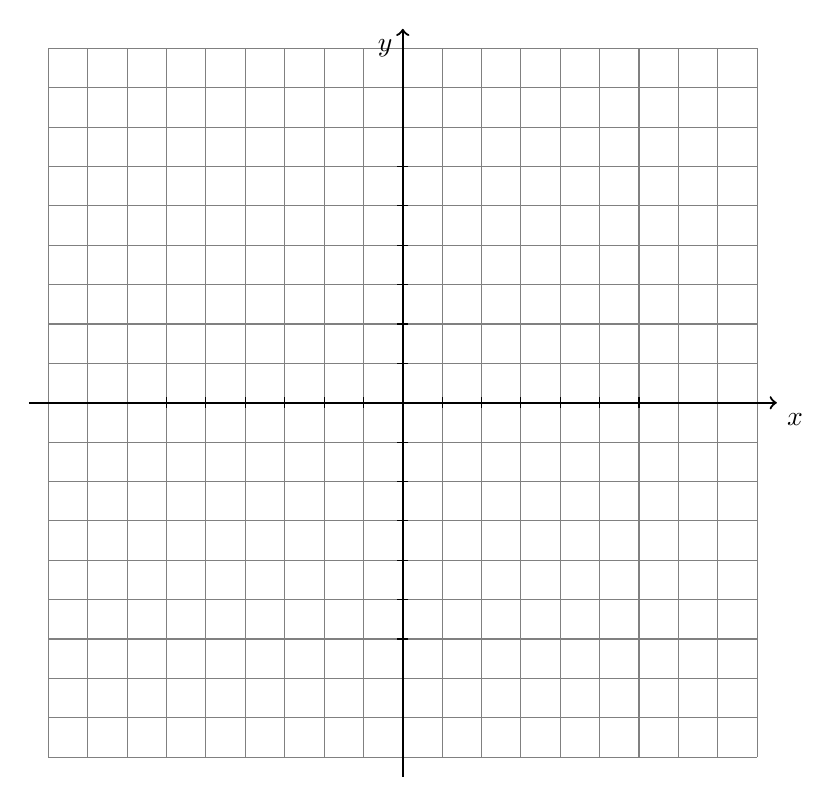
\begin{tikzpicture}[y=.5cm, x=0.5cm,font=\sffamily]
    %% ticks
    \draw[step = 1, gray] (-9,-9) grid (9,9);
    %% axis
    \draw[thick,->] (-9.5,0) -- coordinate (x axis mid) (9.5,0) node[anchor = north west] {$x$};
    \draw[thick,->] (0,-9.5) -- coordinate (y axis mid) (0,9.5) node[anchor = north east] {$y$};
    \foreach \y in {-6,-5,...,-1,1,2,...,6} {
      \draw (2pt, \y) -- (-2pt, \y);
    }
    \foreach \x in {-6,-5,...,-1,1,2,...,6} {
      \draw (\x,2pt) -- (\x,-2pt);
    }

  \end{tikzpicture}

\vfill



\item Graph and label $f(x+2)$ on the coordinate system above.  Then determine the domain and range of $f(x+2)$.

\end{enumerate}
\vfill

\newpage

\item For this problem, let $f(x)=\sqrt{x}$.
\begin{enumerate}
\item Graph $f(x)=\sqrt{x}$.  Then determine the domain and range of $f(x)$.\\
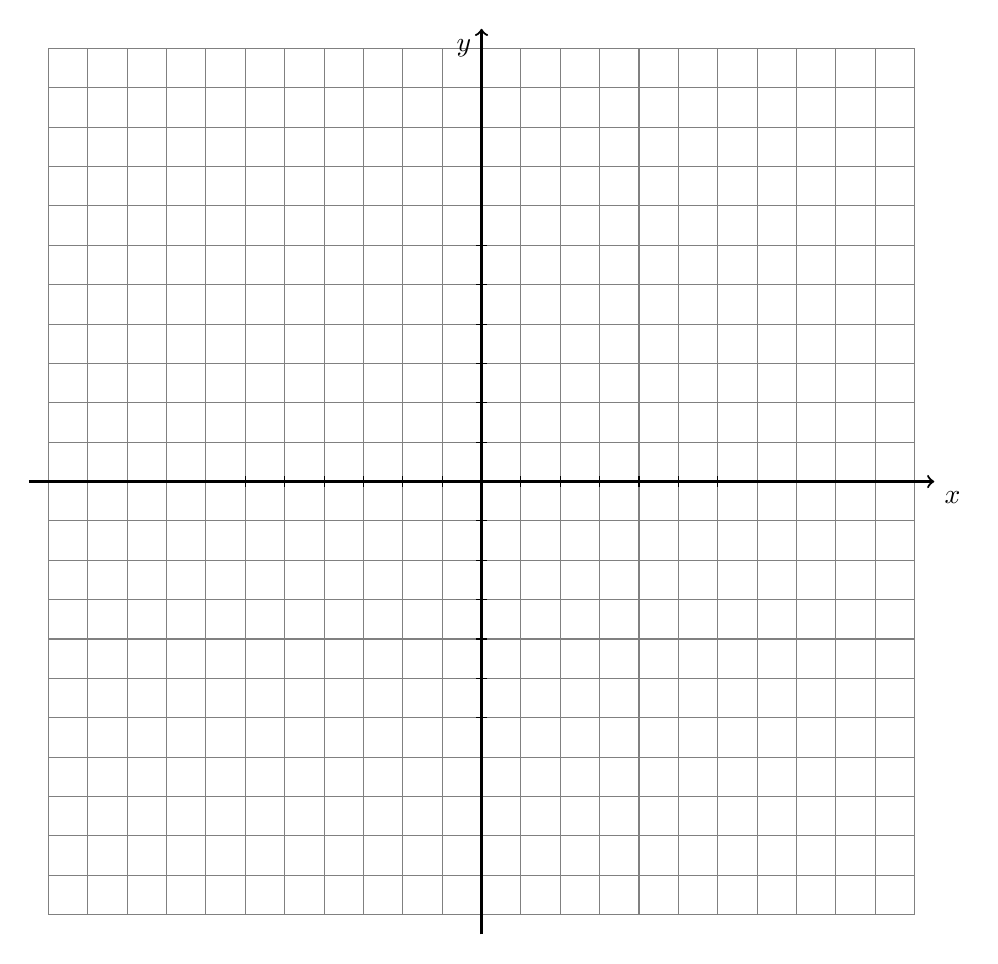
\begin{tikzpicture}[y=.5cm, x=0.5cm,font=\sffamily]
    %% ticks
    \draw[step = 1, gray] (-11,-11) grid (11,11);
    %% axis
    \draw[thick,->] (-11.5,0) -- coordinate (x axis mid) (11.5,0) node[anchor = north west] {$x$};
    \draw[thick,->] (0,-11.5) -- coordinate (y axis mid) (0,11.5) node[anchor = north east] {$y$};
    \foreach \y in {-6,-5,...,-1,1,2,...,6} {
      \draw (2pt, \y) -- (-2pt, \y);
    }
    \foreach \x in {-6,-5,...,-1,1,2,...,6} {
      \draw (\x,2pt) -- (\x,-2pt);
    }

  \end{tikzpicture}

\vfill
\item Graph and label $f(x)-3$ on the coordinate system above.  Then determine the domain and range of $f(x)-3$.\vfill
\vfill
\end{enumerate}






\end{enumerate}



\include{functions/Worksheet-1.6a}

\include{functions/Preclass-1.6B}
\include{functions/Worksheet-1.6b}

\preClass{Coordinate Systems}

\videoLink{Section 1.7}{https://www.youtube.com/playlist?list=PLYHZK3b8UFw0MGYUVN9Z4aYof_QgbFw7f}

\begin{enumerate}

\item  Determine whether the function $f$ is even, odd, or neither.
 $$f(x)=4x^3-x$$


\vfill


\item  Evaluate the function for the given values of $x$.
\[
  g(x) =
  \begin{cases}
                                   x+3 & \text{for $x<-1$} \\
                                   x^2 & \text{for $-1 \leq x <2$}   \end{cases}
\]


\begin{enumerate}
\item $g(-2)=$\\
\item $g(-1)=$\\
\item $g(0)=$\\
\item $g(-5)=$\\


\end{enumerate}
\newpage

\item  Graph the piece-wise defined function.
\[
  h(x) =
  \begin{cases}
    2, & \text{for $x \leq -1$}, \\
    2x, & \text{for $x > -1$}.
  \end{cases}
\]
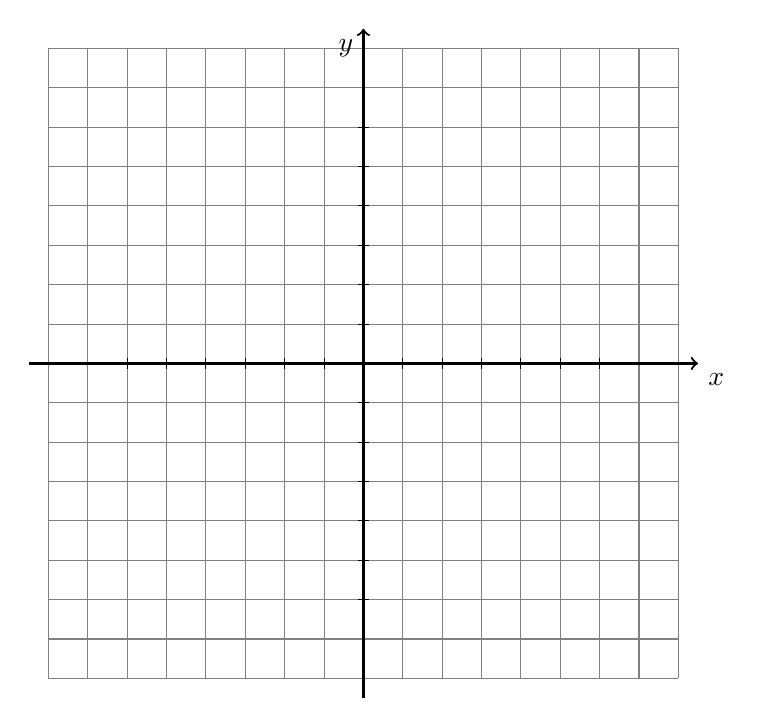
\begin{tikzpicture}[y=.5cm, x=0.5cm,font=\sffamily]
    %% ticks
    \draw[step = 1, gray] (-8,-8) grid (8,8);
    %% axis
    \draw[thick,->] (-8.5,0) -- coordinate (x axis mid) (8.5,0) node[anchor = north west] {$x$};
    \draw[thick,->] (0,-8.5) -- coordinate (y axis mid) (0,8.5) node[anchor = north east] {$y$};
    \foreach \y in {-6,-5,...,-1,1,2,...,6} {
      \draw (2pt, \y) -- (-2pt, \y);
    }
    \foreach \x in {-6,-5,...,-1,1,2,...,6} {
      \draw (\x,2pt) -- (\x,-2pt);
    }
  \end{tikzpicture}



\item  Determine a value of $h$ so that you could sketch the graph of
  the function,
\[
  k(x) =
  \begin{cases}
    h, & \text{for $x \leq -1$}, \\
    2x, & \text{for $x > -1$},
  \end{cases}
\]
without lifting your pencil from the page. Sketch a graph of the
resulting function using the axes below. \\
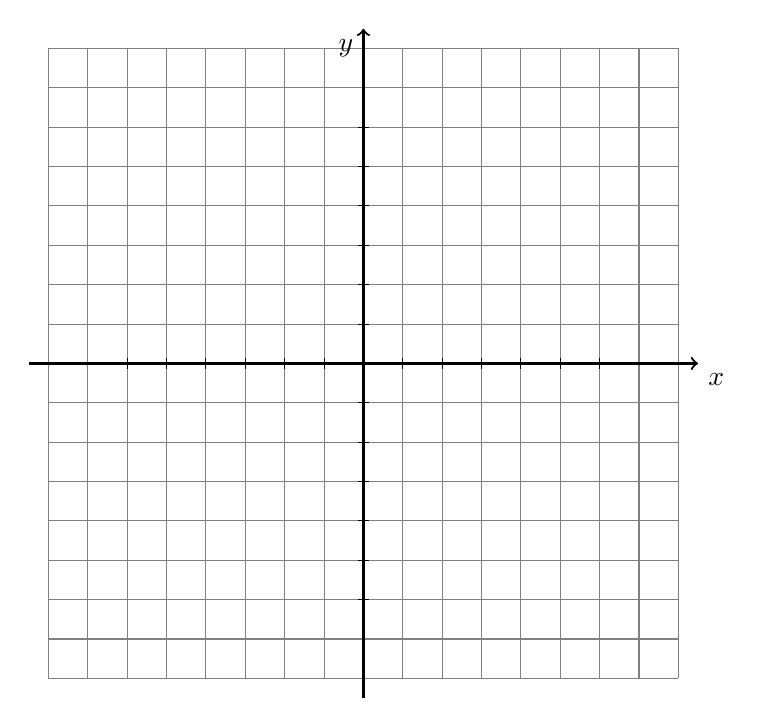
\begin{tikzpicture}[y=.5cm, x=0.5cm,font=\sffamily]
    %% ticks
    \draw[step = 1, gray] (-8,-8) grid (8,8);
    %% axis
    \draw[thick,->] (-8.5,0) -- coordinate (x axis mid) (8.5,0) node[anchor = north west] {$x$};
    \draw[thick,->] (0,-8.5) -- coordinate (y axis mid) (0,8.5) node[anchor = north east] {$y$};
    \foreach \y in {-6,-5,...,-1,1,2,...,6} {
      \draw (2pt, \y) -- (-2pt, \y);
    }
    \foreach \x in {-6,-5,...,-1,1,2,...,6} {
      \draw (\x,2pt) -- (\x,-2pt);
    }

  \end{tikzpicture}







\end{enumerate}





\actTitle{Worksheet 1.7}



\noindent \textbf{Instructions:}  Work together in groups of  3 or 4 to complete the following problems.




\begin{enumerate}
\item Graph each of the following piecewise functions.
\begin{enumerate}
\item \[
  f(x) =
  \begin{cases}
                                   x+5 & \text{if $x<-2$} \\
                                   -4 & \text{if $x \geq 2$}

  \end{cases}
\]

\begin{center}
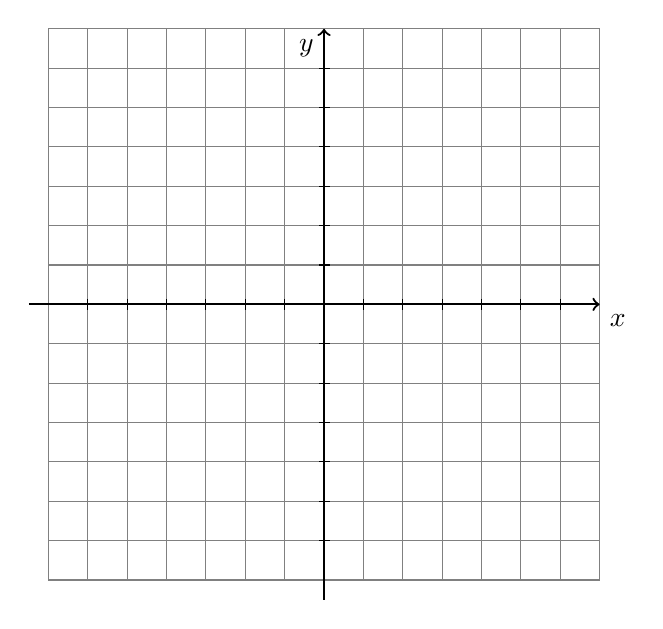
\begin{tikzpicture}[y=.5cm, x=0.5cm,font=\sffamily]
    %% ticks
    \draw[step = 1, gray] (-7,-7) grid (7,7);
    %% axis
    \draw[thick,->] (-7.5,0) -- coordinate (x axis mid) (7,0) node[anchor = north west] {$x$};
    \draw[thick,->] (0,-7.5) -- coordinate (y axis mid) (0,7) node[anchor = north east] {$y$};
    \foreach \y in {-6,-5,...,-1,1,2,...,6} {
      \draw (2pt, \y) -- (-2pt, \y);
    }
    \foreach \x in {-6,-5,...,-1,1,2,...,6} {
      \draw (\x,2pt) -- (\x,-2pt);
    }

\end{tikzpicture}
\end{center}  


\item \[
  f(x) =
  \begin{cases}
                                   2x+1 & \text{if $x<1$} \\
                                   -2x+3 & \text{if $x \geq 1$}

  \end{cases}
\]

\begin{center}
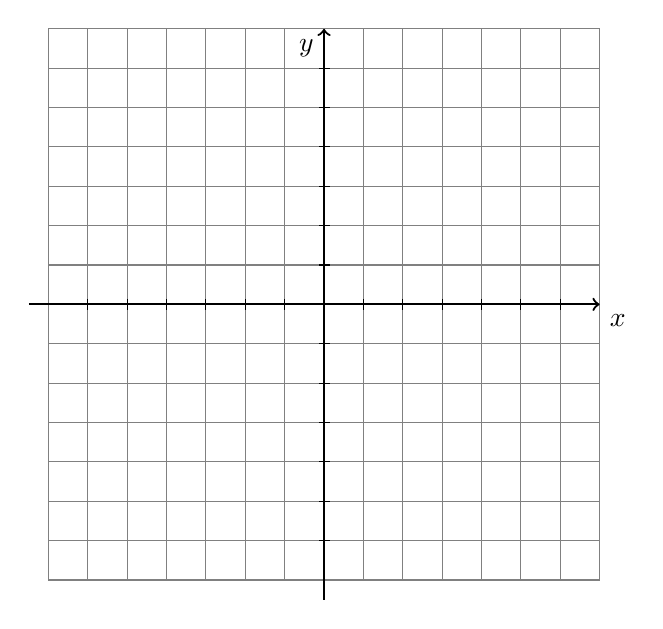
\begin{tikzpicture}[y=.5cm, x=0.5cm,font=\sffamily]
    %% ticks
    \draw[step = 1, gray] (-7,-7) grid (7,7);
    %% axis
    \draw[thick,->] (-7.5,0) -- coordinate (x axis mid) (7,0) node[anchor = north west] {$x$};
    \draw[thick,->] (0,-7.5) -- coordinate (y axis mid) (0,7) node[anchor = north east] {$y$};
    \foreach \y in {-6,-5,...,-1,1,2,...,6} {
      \draw (2pt, \y) -- (-2pt, \y);
    }
    \foreach \x in {-6,-5,...,-1,1,2,...,6} {
      \draw (\x,2pt) -- (\x,-2pt);
    }

\end{tikzpicture}
\end{center}


\newpage

\item \[
  f(x) =
  \begin{cases}
                                   5 & \text{if $x<-2$} \\
                                   \frac{1}{2} & \text{if $-2 \leq x \leq 6$}\\
                                   -2x+10 & \text{if $x > 6$}

  \end{cases}
\]

\begin{center}
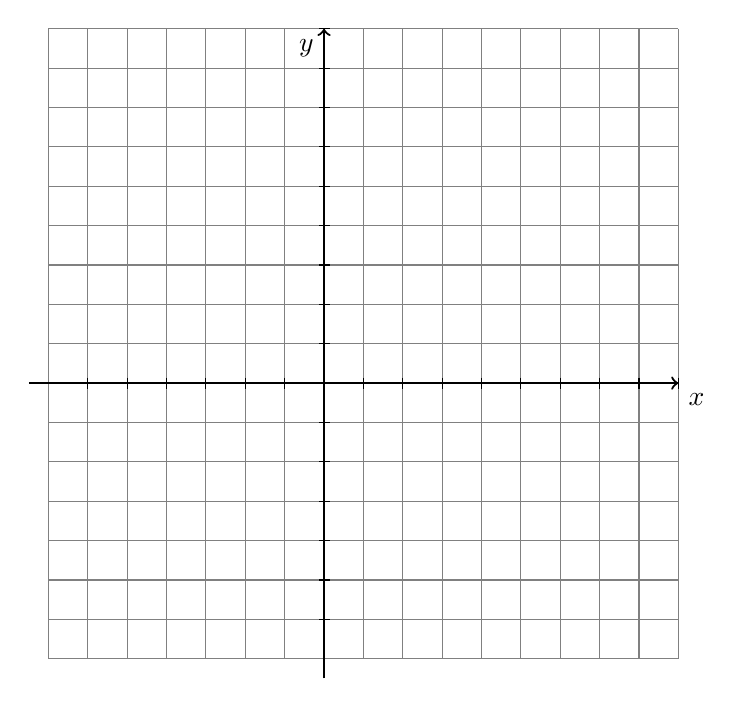
\begin{tikzpicture}[y=.5cm, x=0.5cm,font=\sffamily]
    %% ticks
    \draw[step = 1, gray] (-7,-7) grid (9,9);
    %% axis
    \draw[thick,->] (-7.5,0) -- coordinate (x axis mid) (9,0) node[anchor = north west] {$x$};
    \draw[thick,->] (0,-7.5) -- coordinate (y axis mid) (0,9) node[anchor = north east] {$y$};
    \foreach \y in {-6,-5,...,-1,1,2,...,9} {
      \draw (2pt, \y) -- (-2pt, \y);
    }
    \foreach \x in {-6,-5,...,-1,1,2,...,9} {
      \draw (\x,2pt) -- (\x,-2pt);
    }

\end{tikzpicture}
\end{center}

\end{enumerate}




\item Evaluate the piecewise function for the given values of $x$.
\begin{enumerate}
\item \[
  f(x) =
  \begin{cases}
                                   x+5 & \text{if $x<-2$} \\
                                   -4 & \text{if $x \geq 2$}

  \end{cases}
\]

\vfill

$$f(3)= \quad \quad \quad \quad \quad \quad \quad \quad \quad \quad \quad \quad f(-4)= \quad \quad \quad \quad \quad \quad \quad \quad \quad \quad  f(-2)=\quad \quad$$
\vfill
\item \[
  f(x) =
  \begin{cases}
                                   x-1 & \text{if $x<-2$} \\
                                   2x-1 & \text{if $-2< x \leq 4$}\\
                                   -3x+8 & \text{if $x>4$}

  \end{cases}
\]

\vfill

$$f(-1)= \quad \quad \quad \quad \quad \quad \quad \quad \quad \quad \quad \quad f(-4)= \quad \quad \quad \quad \quad \quad \quad \quad \quad \quad f(5)=\quad \quad $$



\end{enumerate}
\vfill

\newpage 

\item Determine if the function is even, odd, or neither.
\begin{enumerate}
\item $f(x)=4x^2-3|x|$
\vfill
\item $f(x)=4x^3-2x$
\vfill
\item $f(x)=4x^2+2x-3$
\vfill
\end{enumerate}

\newpage

\item Part of the graph of $f(x)$ is shown below. The graph for positive values of $x$ is shown while the portion of the graph for negative values of $x$ is missing.

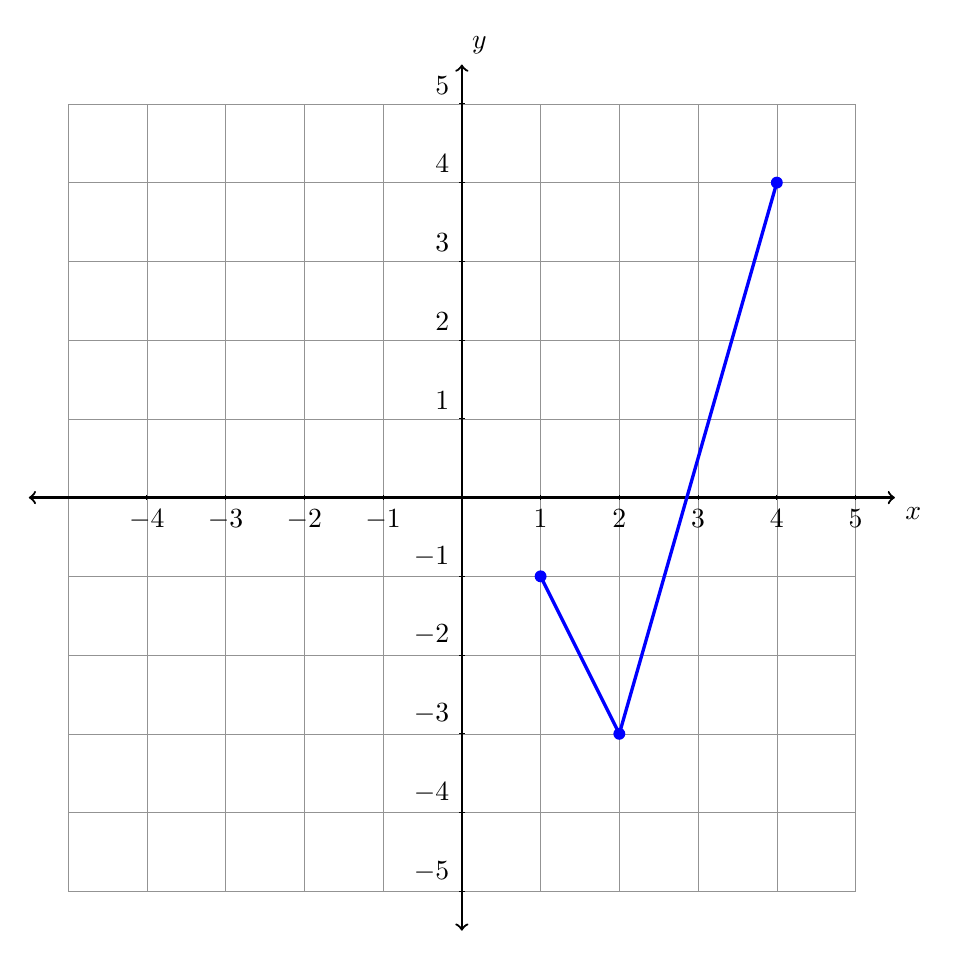
\begin{tikzpicture}[y=1cm, x=1cm,font=\sffamily,
	mydot/.style={
    circle,
    fill=white,
    draw,
    outer sep=0pt,
    inner sep=1.5pt
  }]
    %% Add a grid
    \draw[step = 1, gray, very thin,opacity=0.85] (-5, -5) grid (5, 5);
 	%% Draw the axes
	\draw[thick,<->] (-5.5,0) -- coordinate (x axis mid) (5.5,0) node[anchor = north west] {$x$};
    \draw[thick,<->] (0,-5.5) -- coordinate (y axis mid) (0,5.5) node[anchor = south west] {$y$};
    %% Label the y axis
    \foreach \y in {-5,...,-1,1,2,...,5} {
      \draw (1pt, \y) -- (-1pt, \y) node[anchor = south east] {$\y$};
    }
    %% Label the x axis
    \foreach \x in {-4,...,-1,1,2,...,5} {
      \draw (\x,1pt) -- (\x,-1pt) node[anchor = north] {$\x$};
    }
    %% Draw the function.
    \begin{scope}
         \draw[very thick,blue] (1,-1) -- (2,-3) -- (4,4);
     
    %semi-circle
         %\draw[very thick, blue] (1,1) arc [radius=1, start angle=180, end angle= 5];
     %parabola
     %    \draw[ultra thick, blue, domain=-5:0] plot (\x, {(-0.2)*(\x-5)*(\x+5)});
     %dots
         \fill[blue] (1,-1) circle[radius=0.5ex];
         \fill[blue] (2,-3) circle[radius=0.5ex];
         \fill[blue] (4,4) circle[radius=0.5ex];
      


    \end{scope}

    %%\node[above=0.1cm] at (-2,2 )   {\nextXValue};

\end{tikzpicture}





\begin{enumerate}
	\item Sketch the portion of the graph that is missing given that $f(x)$ is an even function. \vspace{1em}
	\item Using your finished graph from part (a), determine the domain and range of the function $f(x)$. Give your answers in interval notation.
	
	\vspace{1em}
	Domain: \hfill Range: \hfill \phantom{space}
	\vspace{1em}
	
	\item Find the average rate of change of $f(x)$ on the interval $[1,4]$.
	\vfill
\end{enumerate}




\newpage 

\item For each of the following graphs, give equations determining the piecewise function. 

\begin{enumerate}
\item \ 


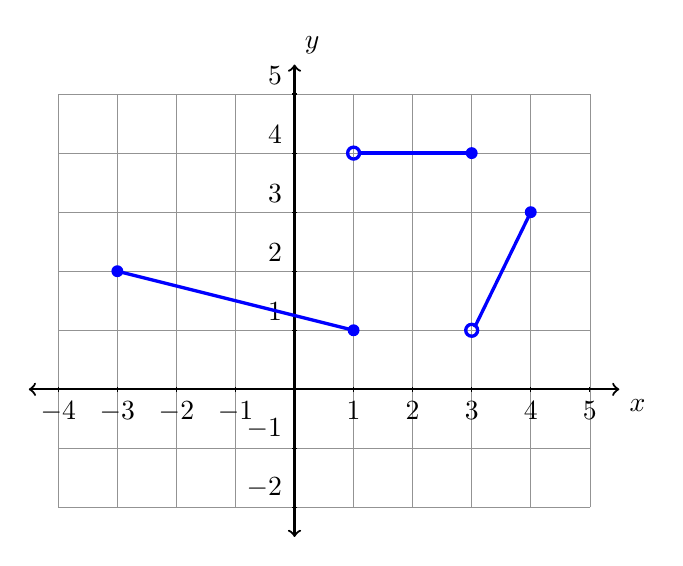
\begin{tikzpicture}[y=.75cm, x=.75cm,font=\sffamily,
	mydot/.style={
    circle,
    fill=white,
    draw,
    outer sep=0pt,
    inner sep=1.5pt
  }]
    %% Add a grid
    \draw[step = 1, gray, very thin,opacity=0.85] (-4, -2) grid (5, 5);
 	%% Draw the axes
	\draw[thick,<->] (-4.5,0) -- coordinate (x axis mid) (5.5,0) node[anchor = north west] {$x$};
    \draw[thick,<->] (0,-2.5) -- coordinate (y axis mid) (0,5.5) node[anchor = south west] {$y$};
    %% Label the y axis
    \foreach \y in {-2,...,-1,1,2,...,5} {
      \draw (1pt, \y) -- (-1pt, \y) node[anchor = south east] {$\y$};
    }
    %% Label the x axis
    \foreach \x in {-4,...,-1,1,2,...,5} {
      \draw (\x,1pt) -- (\x,-1pt) node[anchor = north] {$\x$};
    }
    %% Draw the function.
    \begin{scope}
         \draw[very thick,blue] (-3,2) -- (1,1);
         \draw[very thick,blue] (3.05,1.05) -- (4,3);
         \draw[very thick,blue] (1.1,4) -- (3,4);
    %semi-circle
         %\draw[very thick, blue] (1,1) arc [radius=1, start angle=180, end angle= 5];
     %parabola
     %    \draw[ultra thick, blue, domain=-5:0] plot (\x, {(-0.2)*(\x-5)*(\x+5)});
     %dots
         \fill[blue] (-3, 2) circle[radius=0.5ex];
         \fill[blue] (1,1) circle[radius=0.5ex];
         \fill[blue] (4,3) circle[radius=0.5ex];
         \draw[very thick, blue] (3,1) circle[radius=0.5ex];
         \fill[blue] (3,4) circle[radius=0.5ex];
         \draw[very thick, blue] (1,4) circle[radius=0.5ex];


    \end{scope}

    %%\node[above=0.1cm] at (-2,2 )   {\nextXValue};

\end{tikzpicture}

\vfill

\item \ 

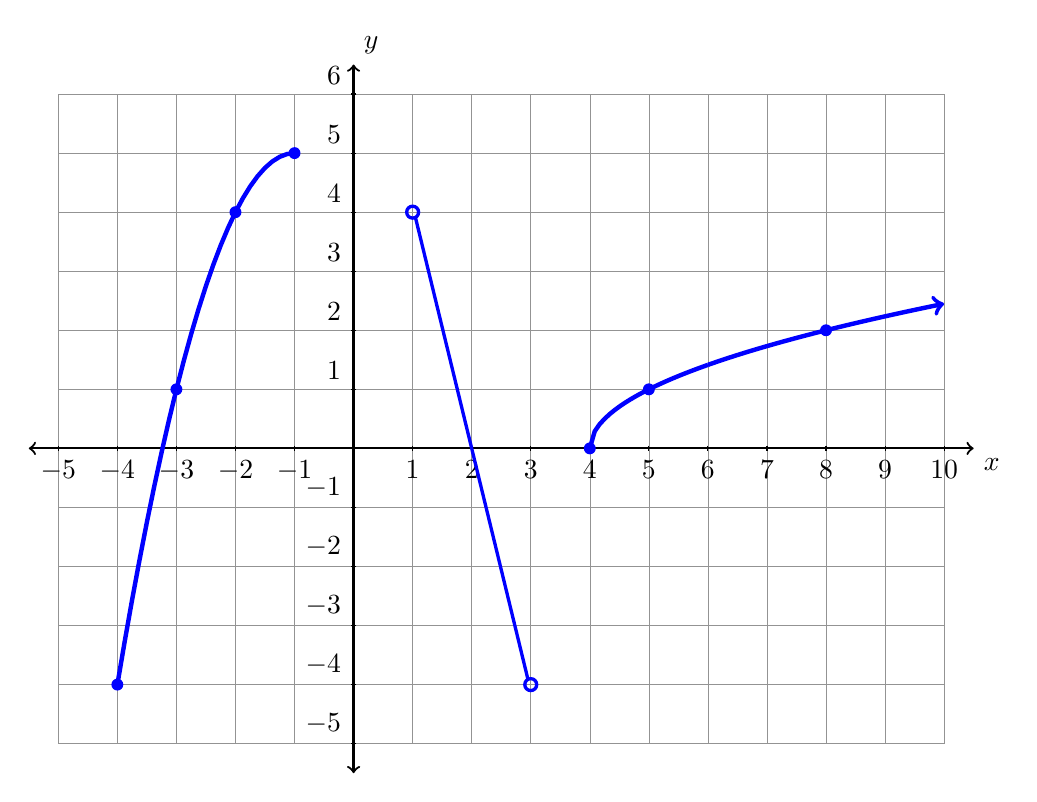
\begin{tikzpicture}[y=.75cm, x=.75cm,font=\sffamily,
	mydot/.style={
    circle,
    fill=white,
    draw,
    outer sep=0pt,
    inner sep=1.5pt
  }]
    %% Add a grid
    \draw[step = 1, gray, very thin,opacity=0.85] (-5, -5) grid (10, 6);
 	%% Draw the axes
	\draw[thick,<->] (-5.5,0) -- coordinate (x axis mid) (10.5,0) node[anchor = north west] {$x$};
    \draw[thick,<->] (0,-5.5) -- coordinate (y axis mid) (0,6.5) node[anchor = south west] {$y$};
    %% Label the y axis
    \foreach \y in {-5,...,-1,1,2,...,6} {
      \draw (1pt, \y) -- (-1pt, \y) node[anchor = south east] {$\y$};
    }
    %% Label the x axis
    \foreach \x in {-5,...,-1,1,2,...,10} {
      \draw (\x,1pt) -- (\x,-1pt) node[anchor = north] {$\x$};
    }
    %% Draw the function.
    \begin{scope}
    %     \draw[very thick,blue] (-3,2) -- (1,1);
       %  \draw[very thick,blue] (3.05,1.05) -- (4,3);
         \draw[very thick,blue] (1.05,3.9) -- (2.95,-3.9);
    %semi-circle
         %\draw[very thick, blue] (1,1) arc [radius=1, start angle=180, end angle= 5];
     %parabola
         \draw[ultra thick, blue, domain=-4:-1] plot (\x, {-(\x+1)^2+5});
         \draw[ultra thick, blue, domain=4:6] plot (\x, {(\x-4)^(1/2)});
         \draw[ultra thick, blue, ->, domain=6:10] plot (\x, {(\x-4)^(1/2)});
     %dots
         \fill[blue] (-4, -4) circle[radius=0.5ex];
         \fill[blue] (-1,5) circle[radius=0.5ex];
         \fill[blue] (-2,4) circle[radius=0.5ex];
         \draw[very thick, blue] (3,-4) circle[radius=0.5ex];
         \fill[blue] (-3,1) circle[radius=0.5ex];
         \fill[blue] (4,0) circle[radius=0.5ex];
         \fill[blue] (5,1) circle[radius=0.5ex];
         \fill[blue] (8,2) circle[radius=0.5ex];

         \draw[very thick, blue] (1,4) circle[radius=0.5ex];


    \end{scope}

    %%\node[above=0.1cm] at (-2,2 )   {\nextXValue};

\end{tikzpicture}

\vfill

\end{enumerate}


\newpage

\item Determine whether or not the following graphs display odd symmetry, even symmetry, or neither.

\begin{multicols}{2}

\begin{enumerate}

\item \ 

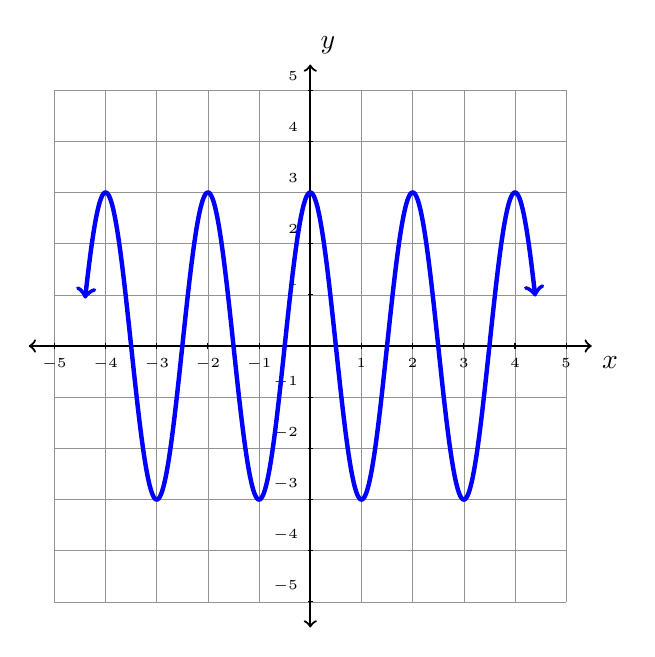
\begin{tikzpicture}[y=.65cm, x=.65cm,font=\sffamily,
	mydot/.style={
    circle,
    fill=white,
    draw,
    outer sep=0pt,
    inner sep=1.5pt
  }]
    %% Add a grid
    \draw[step = 1, gray, very thin,opacity=0.85] (-5, -5) grid (5, 5);
 	%% Draw the axes
	\draw[thick,<->] (-5.5,0) -- coordinate (x axis mid) (5.5,0) node[anchor = north west] {$x$};
    \draw[thick,<->] (0,-5.5) -- coordinate (y axis mid) (0,5.5) node[anchor = south west] {$y$};
    %% Label the y axis
    \foreach \y in {-5,...,-1,1,2,...,5} {
      \draw (1pt, \y) -- (-1pt, \y) node[anchor = south east] {\tiny $\y$};
    }
    %% Label the x axis
    \foreach \x in {-5,...,-1,1,2,...,5} {
      \draw (\x,1pt) -- (\x,-1pt) node[anchor = north] {\tiny $\x$};
    }
    %% Draw the function.
    \begin{scope}
%         \draw[very thick,blue] (-3,2) -- (1,1);
%         \draw[very thick,blue] (3.05,1.05) -- (4,3);
%         \draw[very thick,blue] (1.1,4) -- (3,4);
    %semi-circle
         %\draw[very thick, blue] (1,1) arc [radius=1, start angle=180, end angle= 5];
     %parabola
         %\draw[ultra thick, blue, domain=-5:0] plot (\x, {(-0.2)*(\x-5)*(\x+5)});
         \draw[ultra thick, blue, <->, domain=-4.4:4.4] plot[samples=1000] (\x, {3*cos(pi*\x r)});             %dots
%         \fill[blue] (-3, 2) circle[radius=0.5ex];
%         \fill[blue] (1,1) circle[radius=0.5ex];
%         \fill[blue] (4,3) circle[radius=0.5ex];
%         \draw[very thick, blue] (3,1) circle[radius=0.5ex];
%         \fill[blue] (3,4) circle[radius=0.5ex];
%         \draw[very thick, blue] (1,4) circle[radius=0.5ex];


    \end{scope}

    %%\node[above=0.1cm] at (-2,2 )   {\nextXValue};

\end{tikzpicture}

\item \ 


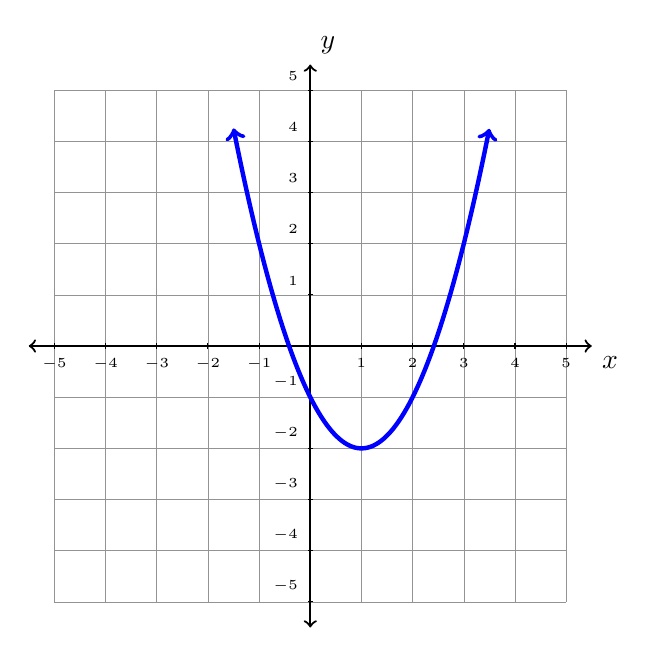
\begin{tikzpicture}[y=.65cm, x=.65cm,font=\sffamily,
	mydot/.style={
    circle,
    fill=white,
    draw,
    outer sep=0pt,
    inner sep=1.5pt
  }]
    %% Add a grid
    \draw[step = 1, gray, very thin,opacity=0.85] (-5, -5) grid (5, 5);
 	%% Draw the axes
	\draw[thick,<->] (-5.5,0) -- coordinate (x axis mid) (5.5,0) node[anchor = north west] {$x$};
    \draw[thick,<->] (0,-5.5) -- coordinate (y axis mid) (0,5.5) node[anchor = south west] {$y$};
    %% Label the y axis
    \foreach \y in {-5,...,-1,1,2,...,5} {
      \draw (1pt, \y) -- (-1pt, \y) node[anchor = south east] {\tiny $\y$};
    }
    %% Label the x axis
    \foreach \x in {-5,...,-1,1,2,...,5} {
      \draw (\x,1pt) -- (\x,-1pt) node[anchor = north] {\tiny $\x$};
    }
    %% Draw the function.
    \begin{scope}
%         \draw[very thick,blue] (-3,2) -- (1,1);
%         \draw[very thick,blue] (3.05,1.05) -- (4,3);
%         \draw[very thick,blue] (1.1,4) -- (3,4);
    %semi-circle
         %\draw[very thick, blue] (1,1) arc [radius=1, start angle=180, end angle= 5];
     %parabola
         %\draw[ultra thick, blue, domain=-5:0] plot (\x, {(-0.2)*(\x-5)*(\x+5)});
         \draw[ultra thick, blue, <->, domain=-1.5:3.5] plot[samples=100] (\x, {(\x-1)^2-2});
           %dots
%         \fill[blue] (-3, 2) circle[radius=0.5ex];
%         \fill[blue] (1,1) circle[radius=0.5ex];
%         \fill[blue] (4,3) circle[radius=0.5ex];
%         \draw[very thick, blue] (3,1) circle[radius=0.5ex];
%         \fill[blue] (3,4) circle[radius=0.5ex];
%         \draw[very thick, blue] (1,4) circle[radius=0.5ex];


    \end{scope}

    %%\node[above=0.1cm] at (-2,2 )   {\nextXValue};

\end{tikzpicture}

\columnbreak

\item \ 

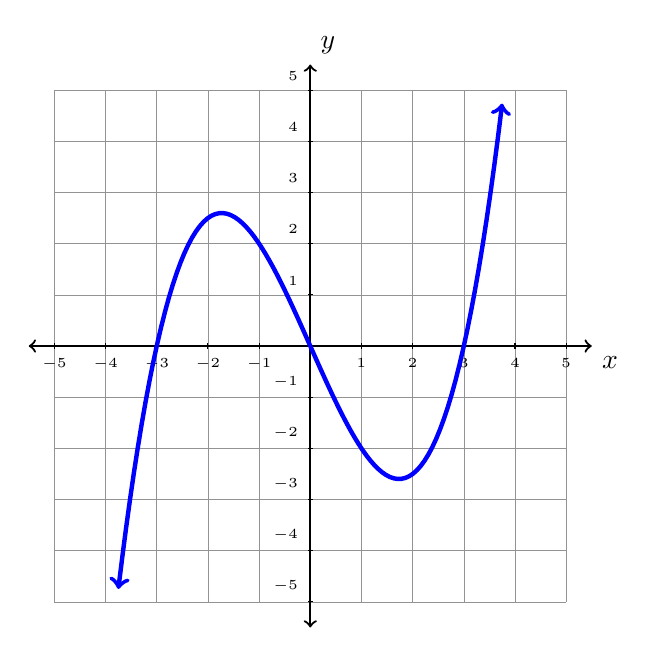
\begin{tikzpicture}[y=.65cm, x=.65cm,font=\sffamily,
	mydot/.style={
    circle,
    fill=white,
    draw,
    outer sep=0pt,
    inner sep=1.5pt
  }]
    %% Add a grid
    \draw[step = 1, gray, very thin,opacity=0.85] (-5, -5) grid (5, 5);
 	%% Draw the axes
	\draw[thick,<->] (-5.5,0) -- coordinate (x axis mid) (5.5,0) node[anchor = north west] {$x$};
    \draw[thick,<->] (0,-5.5) -- coordinate (y axis mid) (0,5.5) node[anchor = south west] {$y$};
    %% Label the y axis
    \foreach \y in {-5,...,-1,1,2,...,5} {
      \draw (1pt, \y) -- (-1pt, \y) node[anchor = south east] {\tiny $\y$};
    }
    %% Label the x axis
    \foreach \x in {-5,...,-1,1,2,...,5} {
      \draw (\x,1pt) -- (\x,-1pt) node[anchor = north] {\tiny $\x$};
    }
    %% Draw the function.
    \begin{scope}
%         \draw[very thick,blue] (-3,2) -- (1,1);
%         \draw[very thick,blue] (3.05,1.05) -- (4,3);
%         \draw[very thick,blue] (1.1,4) -- (3,4);
    %semi-circle
         %\draw[very thick, blue] (1,1) arc [radius=1, start angle=180, end angle= 5];
     %parabola
         %\draw[ultra thick, blue, domain=-5:0] plot (\x, {(-0.2)*(\x-5)*(\x+5)});
         \draw[ultra thick, blue, <->, domain=-3.75:3.75] plot[samples=100] (\x, {(.25)*(\x-3)*(\x)*(\x+3)});
           %dots
%         \fill[blue] (-3, 2) circle[radius=0.5ex];
%         \fill[blue] (1,1) circle[radius=0.5ex];
%         \fill[blue] (4,3) circle[radius=0.5ex];
%         \draw[very thick, blue] (3,1) circle[radius=0.5ex];
%         \fill[blue] (3,4) circle[radius=0.5ex];
%         \draw[very thick, blue] (1,4) circle[radius=0.5ex];


    \end{scope}

    %%\node[above=0.1cm] at (-2,2 )   {\nextXValue};

\end{tikzpicture}

\item \ 

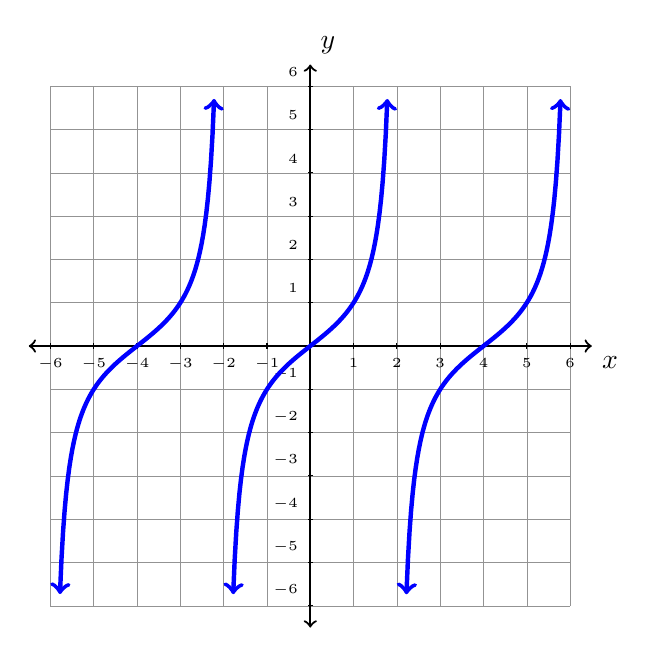
\begin{tikzpicture}[y=.55cm, x=.55cm,font=\sffamily,
	mydot/.style={
    circle,
    fill=white,
    draw,
    outer sep=0pt,
    inner sep=1.5pt
  }]
    %% Add a grid
    \draw[step = 1, gray, very thin,opacity=0.85] (-6, -6) grid (6, 6);
 	%% Draw the axes
	\draw[thick,<->] (-6.5,0) -- coordinate (x axis mid) (6.5,0) node[anchor = north west] {$x$};
    \draw[thick,<->] (0,-6.5) -- coordinate (y axis mid) (0,6.5) node[anchor = south west] {$y$};
    %% Label the y axis
    \foreach \y in {-6,...,-1,1,2,...,6} {
      \draw (1pt, \y) -- (-1pt, \y) node[anchor = south east] {\tiny $\y$};
    }
    %% Label the x axis
    \foreach \x in {-6,...,-1,1,2,...,6} {
      \draw (\x,1pt) -- (\x,-1pt) node[anchor = north] {\tiny $\x$};
    }
    %% Draw the function.
    \begin{scope}
%         \draw[very thick,blue] (-3,2) -- (1,1);
%         \draw[very thick,blue] (3.05,1.05) -- (4,3);
%         \draw[very thick,blue] (1.1,4) -- (3,4);
    %semi-circle
         %\draw[very thick, blue] (1,1) arc [radius=1, start angle=180, end angle= 5];
     %parabola
         %\draw[ultra thick, blue, domain=-5:0] plot (\x, {(-0.2)*(\x-5)*(\x+5)});
         \draw[ultra thick, blue, <->, domain=-1.78:1.78] plot[samples=100] (\x, {tan(.25*pi*\x r)});
         \draw[ultra thick, blue, <->, domain=-5.78:-2.22] plot[samples=100] (\x, {tan(.25*pi*\x r)});
         \draw[ultra thick, blue, <->, domain=2.22:5.78] plot[samples=100] (\x, {tan(.25*pi*\x r)});
           %dots
%         \fill[blue] (-3, 2) circle[radius=0.5ex];
%         \fill[blue] (1,1) circle[radius=0.5ex];
%         \fill[blue] (4,3) circle[radius=0.5ex];
%         \draw[very thick, blue] (3,1) circle[radius=0.5ex];
%         \fill[blue] (3,4) circle[radius=0.5ex];
%         \draw[very thick, blue] (1,4) circle[radius=0.5ex];


    \end{scope}

    %%\node[above=0.1cm] at (-2,2 )   {\nextXValue};

\end{tikzpicture}


\end{enumerate}



\end{multicols}

%\vfill
%
%\item Find a function that is both even and odd.



\item Write the function $f(x) = |x|$ as a piecewise defined function with two linear function pieces.

\vfill

%\newpage 
%\item Use the graph of $y=f(x)$ to answer the following questions.
%\begin{center}
%	\begin{tikzpicture}[y=1cm, x=1cm,font=\sffamily,
%	mydot/.style={
%    circle,
%    fill=white,
%    draw,
%    outer sep=0pt,
%    inner sep=1.5pt
%  }]
%    %% Add a grid
%    \draw[step = 1, gray, very thin,opacity=0.85] (-6, -2) grid (6, 6);
% 	%% Draw the axes
%	\draw[thick,<->] (-6.5,0) -- coordinate (x axis mid) (6.5,0) node[anchor = north west] {$x$};
%    \draw[thick,<->] (0,-2.5) -- coordinate (y axis mid) (0,6.5) node[anchor = south west] {$y$};
%    %% Label the y axis
%    \foreach \y in {-2,...,-1,1,2,...,6} {
%      \draw (1pt, \y) -- (-1pt, \y) node[anchor = south east] {$\y$};
%    }
%    %% Label the x axis
%    \foreach \x in {-6,...,-1,1,2,...,6} {
%      \draw (\x,1pt) -- (\x,-1pt) node[anchor = north] {$\x$};
%    }
%    %% Draw the function.
%    \begin{scope}
%         \draw[very thick,blue] (-3,2) -- (1,1);
%         \draw[very thick,blue] (3.05,1.05) -- (4,3);
%    %semi-circle
%         \draw[very thick, blue] (1,1) arc [radius=1, start angle=180, end angle= 5];
%     %parabola
%     %    \draw[ultra thick, blue, domain=-5:0] plot (\x, {(-0.2)*(\x-5)*(\x+5)});
%     %dots
%         \fill[blue] (-3, 2) circle[radius=0.5ex];
%         \fill[blue] (1,1) circle[radius=0.5ex];
%         \fill[blue] (4,3) circle[radius=0.5ex];
%         \draw[very thick, blue] (3,1) circle[radius=0.5ex];
%
%
%    \end{scope}
%
%    %%\node[above=0.1cm] at (-2,2 )   {\nextXValue};
%
%  \end{tikzpicture}
%\end{center}
%
%
%\begin{enumerate}
%\item Determine the intervals where $f(x)$ is increasing.\vfill
%\item Determine the intervals where $f(x)$ is decreasing.\vfill
%\item Determine the \textbf{location} of any relative minima.\vfill
%\item Determine the \textbf{value} of any relative minima.\vfill
%\item Determine the \textbf{location} of any relative maxima.\vfill
%\item Determine the \textbf{value} of any relative maxima.\vfill
%\end{enumerate}



\end{enumerate}



\preClass{Coordinate Systems}


\videoLink{Section 1.8}{https://www.youtube.com/playlist?list=PLYHZK3b8UFw2GleEiLibLzFIsnrHdy43\_}


\begin{enumerate}

\item Find the following values for the functions $f(x)=|x-3|$, $g(x)=x^3$, $h(x)=\sqrt{x+1}$.
\begin{enumerate}
\item $\displaystyle (f+g)(2)=$
  \vfill
\item $\displaystyle \frac{h}{f}(8)=$
  \vfill
\item $\displaystyle g(h(3))=$
  \vfill
\item $\displaystyle g(f(8))=$
  \vfill
\end{enumerate}

\clearpage

\item  Use $f(x)=x^2+1$ and $g(x)=x+5$ to determine $f(g(x))$ and the domain of $f(g(x))$.
\vfill



\item Given $f(x)=7x+2$.  Determine the difference quotient,
  $\displaystyle \frac{f(x+h)-f(x)}{h}$. Simplify your answer to
  reduce it as much as possible.

\vfill






\end{enumerate}





\actTitle{Worksheet 1.8}



\noindent \textbf{Instructions:}  Work together in groups of  3 or 4 to complete the following problems.




\begin{enumerate}
\item Given $f(x)=5x^2+2x-3$ and $g(x)=x+3$.
\begin{enumerate}
\item Find $(f \circ g)(x)$.
\vfill


\item  Find $(g \circ f)(x)$.
\vfill
 
 \item Find $(f \circ g)(1)$.
 \vfill
 
 \item  Find $(g \circ f)(1)$.
 
 \vfill
 \end{enumerate}

\clearpage

\item Given $f(x)=x^2$ and $g(x)=\sqrt{x}$.
\begin{enumerate}
\item Determine the domains of $f(x)$ and $g(x)$.\vfill
\item Find $(f \circ g)(x)$ and simplify completely.\vfill
\item Determine the domain of $(f \circ g)(x)$.  Keep in mind that the domain of a function is the collection of $x$-values that can be plugged into the function.\vfill
\item  Find $(g \circ f)(x)$ and simplify completely.\vfill
\item Determine the domain of $(g \circ f)(x)$.\vfill
\item What do you notice about $(f \circ g)(x)$ and $(g \circ f)(x)$?  What do you notice about their domains?  Does the domain of the inside function affect the domain of function composition?\vfill
\end{enumerate}




\vfill

\clearpage 

\item Let $f(x)=x^2-1$, $g(x)$ be given by the graph below, and $h(x)$ be given by the table below.


\begin{minipage}[t]{.75\textwidth}
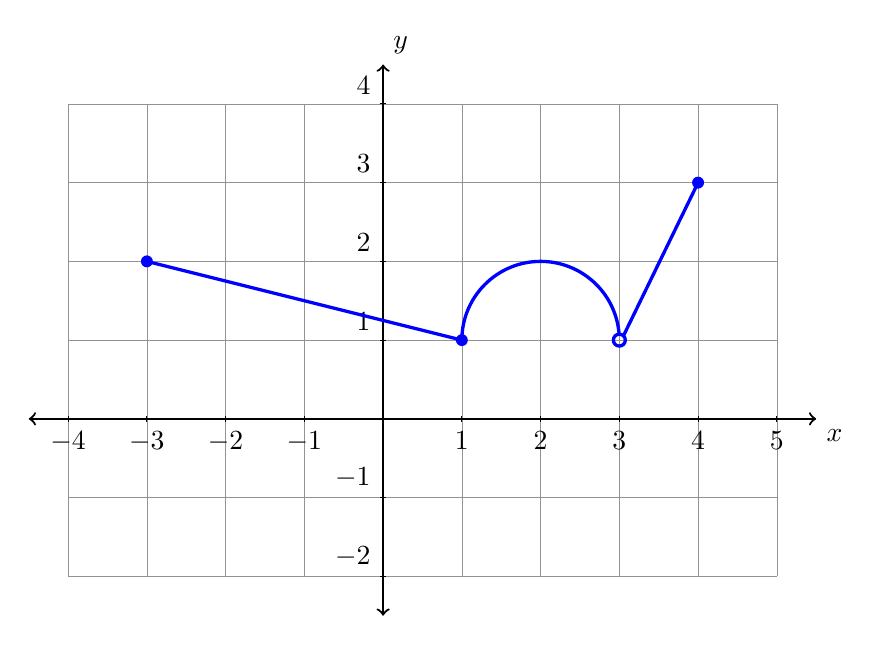
\begin{tikzpicture}[y=1cm, x=1cm,font=\sffamily,
	mydot/.style={
    circle,
    fill=white,
    draw,
    outer sep=0pt,
    inner sep=1.5pt
  }]
    %% Add a grid
    \draw[step = 1, gray, very thin,opacity=0.85] (-4, -2) grid (5, 4);
 	%% Draw the axes
	\draw[thick,<->] (-4.5,0) -- coordinate (x axis mid) (5.5,0) node[anchor = north west] {$x$};
    \draw[thick,<->] (0,-2.5) -- coordinate (y axis mid) (0,4.5) node[anchor = south west] {$y$};
    %% Label the y axis
    \foreach \y in {-2,...,-1,1,2,...,4} {
      \draw (1pt, \y) -- (-1pt, \y) node[anchor = south east] {$\y$};
    }
    %% Label the x axis
    \foreach \x in {-4,...,-1,1,2,...,5} {
      \draw (\x,1pt) -- (\x,-1pt) node[anchor = north] {$\x$};
    }
    %% Draw the function.
    \begin{scope}
         \draw[very thick,blue] (-3,2) -- (1,1);
         \draw[very thick,blue] (3.05,1.05) -- (4,3);
    %semi-circle
         \draw[very thick, blue] (1,1) arc [radius=1, start angle=180, end angle= 5];
     %parabola
     %    \draw[ultra thick, blue, domain=-5:0] plot (\x, {(-0.2)*(\x-5)*(\x+5)});
     %dots
         \fill[blue] (-3, 2) circle[radius=0.5ex];
         \fill[blue] (1,1) circle[radius=0.5ex];
         \fill[blue] (4,3) circle[radius=0.5ex];
         \draw[very thick, blue] (3,1) circle[radius=0.5ex];


    \end{scope}

    %%\node[above=0.1cm] at (-2,2 )   {\nextXValue};

  \end{tikzpicture}
\end{minipage}
%second column
\begin{minipage}[t]{.25\textwidth}
\vspace{-2in}
\begin{tabular}{|l|l|}
\hline
\textbf{$x$} & \textbf{$h(x)$} \\ \hline
-3           & 2               \\ \hline
0            & 4               \\ \hline
1            & 5               \\ \hline
3            & -6              \\ \hline
\end{tabular}
\end{minipage}







\begin{enumerate}
\item Determine the $(f\circ g)(4)$.\vfill
\item Determine the $(g\circ h)(-3)$.\vfill
\item Determine the $(h\circ f)(1)$..\vfill
\item Determine the $(g\circ f)(2)$.\vfill
\end{enumerate}


\clearpage

\item Given $f(x)=4x-9$ and $g(x)=\sqrt{x+6}$
\begin{enumerate}
\item Find $\displaystyle\left(\frac{f}{g}\right)(x)$ and determine its domain.
\vfill
\item Find $\displaystyle\left(\frac{g}{f}\right)(x)$ and determine its domain.
\vfill
\end{enumerate}

\item Given $f(x)=2x^2-5x+1$.  Find the difference quotient, $\displaystyle \frac{f(x+h)-f(x)}{h}$.
\vfill
\vfill



\end{enumerate}






\preClass{Coordinate Systems}

\videoLink{Section 2.1 Day 1}{https://www.youtube.com/playlist?list=PLYHZK3b8UFw1r2QdO6Pgj4jg4-OBM6h1I}


\begin{enumerate}

\item Given $f(x)=4(x+2)^2-4$.
\begin{enumerate}

\item Identify the vertex.
\vfill
\item Determine the $x$-intercept(s).
\vfill
\vfill
\item Sketch the function $f(x)$.\\


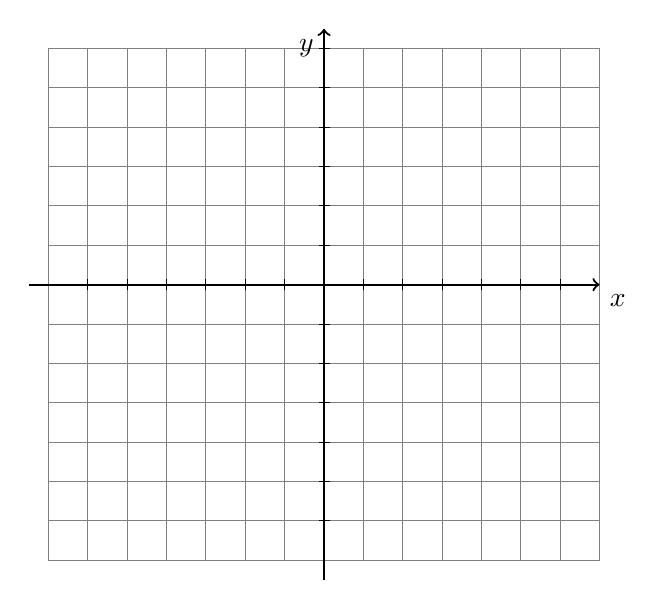
\begin{tikzpicture}[y=.5cm, x=0.5cm,font=\sffamily]
    %% ticks
    \draw[step = 1, gray] (-7,-7) grid (7,6);
    %% axis
    \draw[thick,->] (-7.5,0) -- coordinate (x axis mid) (7,0) node[anchor = north west] {$x$};
    \draw[thick,->] (0,-7.5) -- coordinate (y axis mid) (0,6.5) node[anchor = north east] {$y$};
    \foreach \y in {-6,-5,...,-1,1,2,...,6} {
      \draw (2pt, \y) -- (-2pt, \y);
    }
    \foreach \x in {-6,-5,...,-1,1,2,...,6} {
      \draw (\x,2pt) -- (\x,-2pt);
    }

\end{tikzpicture}



\item Determine an equation for the axis of symmetry.
\end{enumerate}



\vfill
\newpage

\item  Complete the square and use that work to find the vertex of the graph of the quadratic function.
$$y=5x^2-30x+49$$

%\item  You have a 500 foot roll of fencing and a large field.  You want to construct a rectangular playground area.  What are the dimensions of the largest such playground?  What is the largest area?
%\begin{enumerate}
%\item Draw a picture of the rectangular playground and label the side lengths using your own variables.
%\vfill
%\vfill
%\item Using your variables, write an equation that represents the area of the playground.
%\vfill
%\item Your previous answer should have two variables.  Use 500 to represent the perimeter of the the playground and solve for one of your variables.  (Note: all four sides of the rectangle will be used.)
%\vfill
%\vfill
%\item Rewrite your area equation in terms of only one variable and simplify.  The result should be a quadratic function.
%\vfill
%
%
%\newpage
%
%
%
%\item To determine the maximum area possible for the playground, what part of the parabola do you need to locate?
%\vfill
%
%\item Find that part of the parabola (from your previous answer).
%\vfill
%\vfill
%\item What is the largest area the playground could be?
%\vfill
%
%\item  What are the dimensions of that playground?
%\vfill
%
%\end{enumerate}
%
%
%




\end{enumerate}



\include{functions/Worksheet-2.1a}

\preClass{Coordinate Systems}


\videoLink{Section 2.1 Day 2}{https://www.youtube.com/playlist?list=PLYHZK3b8UFw3qJR_5u0E1b2wuXCeuCBIX}


\begin{enumerate}

\item   You have a 500 foot roll of fencing and a large field.  You want to construct a rectangular playground area.  What are the dimensions of the largest such playground?  What is the largest area?
\begin{enumerate}
\item Draw a picture of the rectangular playground and label the side lengths using your own variables.
\vfill
\vfill
\item Using your variables, write an equation that represents the area of the playground.
\vfill
\item Your previous answer should have two variables.  Use 500 to represent the perimeter of the the playground and solve for one of your variables.  (Note: all four sides of the rectangle will be used.)
\vfill
\vfill
\item Rewrite your area equation in terms of only one variable and simplify.  The result should be a quadratic function.
\vfill


\newpage



\item To determine the maximum area possible for the playground, what part of the parabola do you need to locate?
\vfill

\item Find that part of the parabola (from your previous answer).
\vfill
\vfill
\item What is the largest area the playground could be?
\vfill

\item  What are the dimensions of that playground?
\vfill

\end{enumerate}







\end{enumerate}




\include{functions/Worksheet-2.1b}


\actTitle{Worksheet Problem Solving}

\noindent \textbf{Instructions:}  Work together in groups of  3 or 4 to complete the following problems.


\begin{enumerate}



\item The value of a newly purchased equipment is a linear function of time. A company purchases a piece of equipment for \$40,000. After 5 years, the equipment loses 15\% of its value. Answer the following:

\begin{enumerate}
\item Determine the value of the equipment after 5 years.
\item Express the value V (in dollars) of the equipment as a function of time t (in years) since purchase.
\item Determine the total time (in years) it will take for the machine to be worth 45\% of its original value.
\end{enumerate}

\vfill

\item Give the coordinates of all of the points that lie on \emph{both} the parabola $y=x^2+1$ \emph{and} the line $y=2x+4$.  Use the following steps to answer the question.
	\begin{enumerate}
		\item How can one describe an arbitrary point on the line $y=2x+4$ as an ordered pair?
		\item How can one describe an arbitrary point on the line $y=x^2+1$ as an ordered pair?
		\item How do these descriptions help you find the intersection.
	\end{enumerate}

\vfill
\newpage


\item You have 50 cm of wire, and you have to use part of this wire to
make a rectangle that's twice as long as it is wide, and the rest of the wire (if there
is any left) to make a square.
What should the dimensions of the shapes be if you want the total area to be as
small as possible? 

\newpage

\item Find the point $(x,y)$ lying on the parabola $y = x^2 + 2x + 1$ so that the average rate of change on the interval between $x$ and $2$ is zero.

\vfill

\item On the coordinate axes below, draw a function whose domain is
	$$[-2,1]\cup(2,3]\cup\{5\}$$
	and whose range is
	$$[-6,-4)\cup[-1,1]\cup\{2\}\cup(3,4].$$

\begin{center}
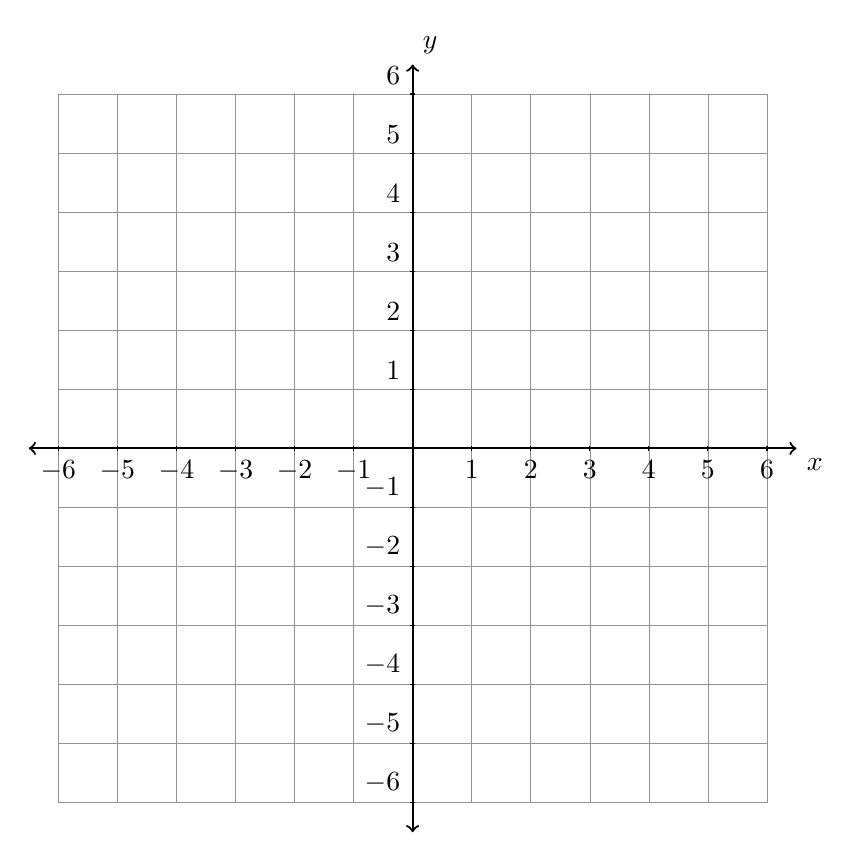
\begin{tikzpicture}[y=.75cm, x=.75cm,font=\sffamily,
	mydot/.style={
    circle,
    fill=white,
    draw,
    outer sep=0pt,
    inner sep=1.5pt
    }]
    %% Add a grid
    \draw[step = 1, gray, very thin,opacity=0.85] (-6, -6) grid ( 6, 6);
 	%% Draw the axes
	\draw[thick,<->] (-6.5,0) -- coordinate (x axis mid) (6.5,0) node[anchor = north west] {$x$};
    \draw[thick,<->] (0,-6.5) -- coordinate (y axis mid) (0,6.5) node[anchor = south west] {$y$};
    %% Label the y axis
    \foreach \y in {-6,...,-1,1,2,...,6} {
    	\draw (1pt, \y) -- (-1pt, \y) node[anchor = south east] {$\y$};
    }
    %% Label the x axis
    \foreach \x in {-6,...,-1,1,2,...,6} {
    	\draw (\x,1pt) -- (\x,-1pt) node[anchor = north] {$\x$};
    }
    %% Draw the function.
%    \begin{scope}
%         \draw[scale=1.0,very thick,black] (-2, 0) -- (1,-2);
%         \draw[scale=1.0,very thick,black] (1.05,1.04) -- (3,2);
%         \fill[black] (-2, 0) circle[radius=0.5ex];
%         \fill[black] (3,2) circle[radius=0.5ex];
%         \fill[black] (1,-2) circle[radius=0.5ex];
%         \draw[scale=1.0, very thick, black] (1,1) circle[radius=0.5ex];
%    \end{scope}

    %%\node[above=0.1cm] at (-2,2 )   {\nextXValue};

\end{tikzpicture}
\end{center}




\newpage

\item Find the point $P$ on the graph of $\sqrt{x}$ such that the line through $P$ and $(1,1)$ has slope $\displaystyle \frac{4}{7}$.
\vfill




\item A business forms a model of its widget sales via a pricing function $p(x) = 400-\frac{70}{8}x$. Here, $x$ is the number of widgets sold and $p(x)$ is the sales price in dollars per widget.  
\begin{enumerate}
\item Find the revenue function $R(x)$ for this business (revenue is total sales). 
\item Find the number $x$ sold that will maximize revenue. (This will be an unrealistic fraction,
but do not round.)
\item What is the maximum revenue? 
\item What is the price $p(x)$ that yields maximum revenue?
\end{enumerate}

\vfill
\vfill



%\newpage
%
%
%\newpage
%
%\item A small business makes scarves and sells them at the farmer's market.  The fixed monthly cost for the rental space at the farmer's market is \$200.  The cost of labor and supplies for the scarves amounts to \$7 per scarf, which are sold for \$35 each at the market.
%\begin{enumerate}
%\item Write a linear functions for the cost $C(x)$, revenue $R(x)$, and profit $P(x)$ corresponding to the production/sale of $x$ scarves per month.
%\vfill
%\item Determine the cost, revenue, and profit associated with selling 15 scarves in one month. Will the business make a profit or lose money that month?
%\vfill
%\item Determine the least number of scarves that must be produced and sold for a monthly profit.  Your answer should be an appropriate whole number.

%\end{enumerate}
%
%\vfill


%\newpage
%
%
%\vfill
%
%\item A diverter at the end of a gutter spout is meant to direct water away from a house.  The homeowner makes the diverter from a rectangular piece of aluminum that is 20 inches long and 12 inches wide.  She makes two folds both parallel to the 20 inch side.  Each fold is a distance \(x\) inches away from the edge.  
%\begin{enumerate}
%\item Write the volume of water that can be carried through the diverter as a function of \(x\).
%\item What is the maximum volume of water that can be carried through the diverter?
%\end{enumerate}  
%
%\vfill





\end{enumerate}





%%% Local Variables:
%%% mode: latex
%%% TeX-master: "../labManual"
%%% End:
